\documentclass[11pt]{article}
\usepackage[review]{acl}
\usepackage{times,latexsym}
\usepackage[T1]{fontenc}
\usepackage[utf8]{inputenc}
\usepackage{microtype,inconsolata}
\usepackage{graphicx,booktabs,amsmath,amssymb,multirow,longtable,array}
\title{Do Language Models Have Medical Beliefs?\\Tracing Evidence, Internal Disease Information, and Diagnostic Choice}
\author{Anonymous ACL submission}
\begin{document}
\maketitle
\begin{abstract}
When clinical evidence changes, does a language model revise a disease representation that actually governs its diagnosis? We study this question by separating diagnostic output, internally decodable disease information, and the causal effect of that information. Using 120 held-out synthetic patients spanning 24 diseases, we follow all evidence prefixes for 24 patients and inspect every layer of two Qwen3 configurations. Presenting identical patient facts as a fixed questionnaire improves final-layer disease decoding in the 1.7B model from 100/120 to 112/120, while its own 24-disease ranking deteriorates from 56/120 to 14/120. Continuous internal and output updates remain positively associated, but their association weakens under the questionnaire. Directions learned from other patients causally increase target-disease scores in all eight primary contrasts, yet produce no additional correct diagnoses at the tested dose. Case-complete analyses reveal recovery, relapse, stable error, and counterexamples where the model outperforms its readout. A 4B configuration reproduces the decoding--diagnosis gap and presentation sensitivity. These findings characterize medical belief through the relationship between information, updating, and decision-making: disease information is available and causally consequential, but does not reliably determine the final diagnosis.
\end{abstract}

\section{Introduction}
A patient has right-ear pain, recent oral antibiotic treatment for an ear infection, and fever. When these facts are revealed sequentially, a language model changes its answer to acute otitis media after the treatment history arrives and retains that diagnosis. Put the same facts into a questionnaire whose remaining entries explicitly say \emph{Unknown}, and the model instead selects acute exacerbation or infection of chronic obstructive pulmonary disease (COPD). A readout trained on other patients can nevertheless identify otitis media from its later layers.

What, then, is the model's medical belief? Its answer suggests one disease; its internal representation supports a classifier predicting another. Neither observation alone resolves the question. The answer can depend on the output interface, and the readout can learn a classification rule that the original model does not use. A useful investigation must follow what evidence changes \emph{inside} the model and whether those changes affect its own diagnostic choice.

Belief updating and medical representation analysis already have direct precedents. DeReLab measures defeasible belief revision and confirmation bias with turn-level ground truth \citep{derelab}. Clinical studies examine changes in judgments over patient trajectories \citep{zeng2026}, while diagnostic coherence tests examine stated distributions under evidence transformations \citep{arun2026}. Medical knowledge maps analyze intermediate activations and perform layer lesions and activation patching \citep{marinescu2025}. Our question connects these strands: \textbf{how tightly are evidence-responsive disease information and diagnostic choice coupled within the same patient trajectory?}

We examine three levels. First, \emph{expressed support}: which disease name does the model favor after each evidence group? Second, \emph{represented information}: which disease can be decoded from each layer, and how do its scores change? Third, \emph{causal influence}: does intervening on a disease-related direction move the original model's scores, and does it change the diagnosis? We use ``medical belief'' as the object investigated through these relationships, not as an assumed hidden probability distribution.

The opening example motivates a population-level result. On 120 held-out patients, a fixed questionnaire raises 1.7B final-layer readout accuracy but sharply reduces native diagnostic ranking. This is not universal: some patients improve under the questionnaire, some diagnoses are correct despite an incorrect readout, and some fail in both channels. We therefore provide all 24 deeply measured trajectories, rather than defining the phenomenon through selected successes.

Our contributions are three empirical connections. (1) We join sequential diagnostic behavior to layerwise disease decoding on disjoint patients. (2) We link natural score updates to controlled disease-direction interventions, distinguishing a score effect from a corrected decision. (3) We separate semantic answers, evidence presentation, candidate ordering, and intervention position, and replicate the central discrepancy in a second model configuration. Together these experiments support a conditional account: disease information can be preserved and affect generation without reliably controlling diagnosis.

\begin{figure*}[t]
\centering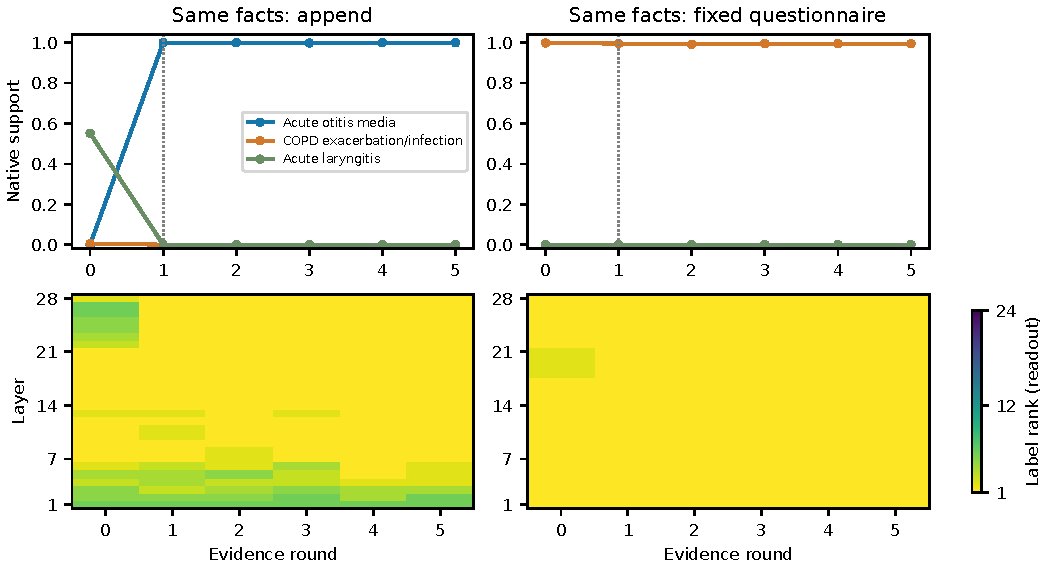
\includegraphics[width=.92\textwidth]{figures/opening_case.pdf}
\caption{One patient, identical facts, different diagnostic trajectories. The source label is acute otitis media. Round 1 reveals recent oral antibiotic treatment for an ear infection; subsequent groups add fever, cough, vaccination status, and travel history. Top: native disease-name support. Bottom: the source label's rank in independent-patient layer readouts (yellow is rank 1). Readout ranks are not native disease probabilities. This post-hoc illustrative case motivates the all-patient analyses.}\label{fig:opening}
\end{figure*}

\section{What Would Count as a Medical Belief?}
\label{sec:belief}
We evaluate a candidate disease state along three axes rather than assigning belief to a single activation or attention map.

\paragraph{Content.} A state should distinguish competing diseases for a patient. We measure decodability using linear readouts trained only on other patients. This tests informational availability; it does not establish that the model has already inferred the decoded diagnosis. Probing accuracy need not imply task relevance \citep{probing}, and probes can learn from retained contextual features \citep{contextprobe}.

\paragraph{Updating.} The state should respond to new patient evidence. We compare disease-pair score changes in the readout and the original model, holding the pair fixed within each update. A stable top disease can conceal substantial changes in relative support. Conversely, a small score crossing can change the top disease. We therefore report continuous updates and discrete switches separately.

\paragraph{Influence on choice.} Disease-related state variation should affect the model's own output. We intervene along readout-derived directions, compare target, opposite, random, and zero directions, and measure the original model's complete disease-name scores. Causal influence on a score is weaker than sufficient influence to change the selected diagnosis. We measure both.

These axes yield three research questions: \textbf{RQ1}, what patterns of diagnostic revision occur as evidence accumulates? \textbf{RQ2}, how do those revisions relate to internal disease information across layers? \textbf{RQ3}, when does disease-related internal information influence the model's diagnostic decision? Presentation and model configuration serve as controlled conditions under which these relationships may change. The study does not test subjective experience or a human-like commitment to an earlier answer.

\section{Experimental Design}
\label{sec:design}
\paragraph{Patients and reference diagnoses.}
We use DDxPlus, a synthetic clinical corpus with symptoms, antecedents, pathology labels, and reference differentials \citep{ddxplus}. Readouts are trained on an existing 120-patient validation cohort. Evaluation uses 120 patients from the official test split, five for each of 24 diseases across six disease groups. Selection uses fixed hashes, ages 18--90, at least five evidence groups, and exclusion of exact fact-set duplicates with previous cohorts, ignoring age and sex. Both splits still share the same simulator.

An independently hashed subset of 24 test patients, covering 17 diseases and all six groups, receives complete prefix measurement: 208 prefixes and 184 evidence additions per presentation. This subset was selected before observing its model outputs. The final pathology label is the endpoint reference. It is also the top reference-differential diagnosis for 79/120 patients. No unique ground-truth posterior is available for intermediate prefixes; leaving the final label early is not automatically an unreasonable clinical update.

\paragraph{Evidence presentation.}
The initial prefix contains one source evidence group. Each subsequent round adds a source group, potentially containing related fields such as pain location and severity. The order is fixed by hash. Every prefix is a fresh forward pass over cumulative evidence, with no previous model answer. Rounds indicate information acquisition, not physiological disease progression.

In \emph{append} input, only revealed question--answer pairs are shown. In the \emph{fixed panel}, all 223 question fields are visible; unrevealed answers are marked Unknown, explicitly distinguished from No. Facts are matched, but length, positions, and unknown-field context differ. Follow-ups relocate known facts, remove Unknown rows, alter one Yes/No answer, and reorder candidates. The mask of which answers are known remains potentially informative even when every question is visible.

\paragraph{Models and captures.}
We use Qwen3-1.7B in FP16 and an existing Qwen3-4B 8-bit configuration \citep{qwen3}. Explicit thinking is disabled. All weights remain frozen. We record all 28/36 layers at the diagnostic anchor, including incoming residual, attention increment, post-attention residual, MLP increment, and outgoing residual. We also reconstruct anchor attention by head and input group. This captures anchor-to-input attention, not every token-to-token attention matrix. Size and precision differ together; the second configuration is a replication, not an isolated scaling experiment.

\paragraph{Native support.}
For a fixed JSON prefix, let $y(d)$ contain the canonical disease name, closing syntax, and EOS. We compute
\begin{align}
 L_t(d)&=\sum_j\log P_\theta(y_j(d)\mid E_t,y_{<j}(d)),\\
 q_t(d)&=\frac{\exp L_t(d)}{\sum_{k\in D}\exp L_t(k)}.
\end{align}
The main candidate universe $D$ contains 49 names. $q$ is relative support among these strings, not a calibrated clinical posterior. We retain per-token scores, canonical-string mass, mean-token scores, and greedy continuations. For comparison with 24-class readouts, we also rerank the 24 sampled diseases within the same 49-name prompt. An actual 24-candidate prompt is tested separately.

\paragraph{Layer readouts.}
For each layer $\ell$, normalize its outgoing anchor state $u=h/\lVert h\rVert_2$ and fit centered ridge regression to one-hot training labels:
\begin{equation}
 s_\ell(u)=(u-\mu_\ell)W_\ell+b.
\end{equation}
There are 24 output classes; ridge strength is 0.1, with 0.01 and 1 sensitivity checks. Heads are fitted independently by layer, presentation, and model, using only old-patient endpoints. Test prefixes never train the heads. Readout scores are not probabilities, and their supervision differs from that of the unadapted native model.

\paragraph{Inference and provenance.}
Patients, not tokens or rounds, are statistical units. Trajectory statistics are first aggregated within patient. We use 2,000 patient-bootstrap replicates for descriptive 95\% intervals, exact binomial boundary intervals for all-zero/all-one binary outcomes, and 20,000 paired sign permutations with Holm correction for eight prespecified intervention contrasts. Fixed-head intervals do not include readout-training uncertainty. Presentation and candidate follow-ups reuse the 24 patients and are exploratory. Appendix~\ref{app:repro} gives implementation checks and the analysis chronology.

\section{RQ1: How Does Diagnostic Support Change?}
\label{sec:behavior}
\paragraph{Abrupt revision and persistent error coexist.}
Across 184 updates, the 1.7B append model changes its top-49 disease 77 times; 69 updates change at least one disease's support by 0.5 or more. The fixed panel has 23 switches and 21 large updates. The 4B append configuration has 55 and 53 respectively. These counts distinguish argmax changes from large shifts; their overlap is not assumed.

To make the range visible, we classify all trajectories by their relationship to the source label (Table~\ref{tab:patterns}). The taxonomy is a post-hoc descriptive analysis of frozen records. ``Recover'' means an earlier label hit was followed by a departure and then a correct endpoint; ``lose'' means the label was hit but not selected at the endpoint. Cases that never hit it are split by whether their top disease changes. The categories are mutually exclusive and exhaustive.

\begin{table}[t]
\centering\small
\begin{tabular}{lrrr}\toprule
Trajectory type & 1.7B A & 1.7B P & 4B A\\\midrule
Always hits source label & 0 & 0 & 2\\
Acquires and retains & 5 & 3 & 8\\
Departs, then recovers & 6 & 0 & 6\\
Hits label, ultimately loses & 5 & 5 & 3\\
Never hits, fixed answer & 1 & 10 & 0\\
Never hits, changes & 7 & 6 & 5\\\bottomrule
\end{tabular}
\caption{All 24 trajectories per condition; A: append, P: fixed panel. These describe source-label agreement, not per-round clinical validity.}\label{tab:patterns}
\end{table}

The panel's lower switch count is therefore not evidence of better belief stability. Ten patients retain one incorrect disease throughout, compared with one under append input. Conversely, genuine endpoint recovery is common under append input: six patients in each model return to the source label after departing from it.

\paragraph{Contrasting cases.}
Otitis media illustrates acquisition followed by retention. Pancreatic neoplasm illustrates repeated entry and exit: the 1.7B append model selects pancreatic neoplasm twice, but ends at bronchiolitis while the final-layer readout identifies pancreatic neoplasm. Acute dystonic reactions provide a stable-error case: one trajectory remains at acute laryngitis despite a final readout selecting the source label. These are distinct forms of failure, not interchangeable examples of one monotonic drift.

Counterexamples are equally important. For Boerhaave syndrome, the native endpoint is correct while the final-layer readout predicts GERD. A pulmonary-embolism patient ends with an incorrect native diagnosis and an incorrect readout. An anemia patient is misclassified under append input but correctly classified under the panel. A pneumothorax patient is correctly classified under both. Ten contrasting examples are plotted in Appendix~\ref{app:examples}, and every evidence group and output is listed for all 24 patients in Appendix~\ref{app:cases}.

\paragraph{Order affects endpoints.}
With complete facts retained, reversing their append order changes the 1.7B top diagnosis for 9/24 patients; a fixed shuffle changes it for 6/24. This establishes order sensitivity under the tested prompts, without establishing which intermediate ordering is clinically preferable. The presentation comparisons below keep the patient facts matched and examine how the resulting diagnostic behavior relates to internal information.

\section{RQ2: Does Internal Information Track Diagnosis?}
\label{sec:representation}
\paragraph{Availability and choice separate.}
Table~\ref{tab:main} compares native ranking and readouts over the same 24 diseases. In 1.7B append input, the final-layer readout identifies 100/120 labels, against 56/120 for native ranking. With the panel, readout accuracy rises to 112/120 while native ranking falls to 14/120. The paired readout-minus-native differences are 36.7 percentage points (95\% CI [27.5,46.7]) and 81.7 [74.2,88.3]. The comparison quantifies different outputs under different supervision, rather than an unsupervised diagnostic improvement.

\begin{table}[t]
\centering\small
\begin{tabular}{lrrr}\toprule
Configuration & Native 49 & Native 24 & Last readout\\\midrule
1.7B append & 44/120 & 56/120 & 100/120\\
1.7B panel & 10/120 & 14/120 & 112/120\\
4B append & 75/120 & 82/120 & 110/120\\\bottomrule
\end{tabular}
\caption{Endpoint source-label matches. Native 24 reranks the sampled classes within the 49-name prompt. Readouts are trained on 120 separate patients.}\label{tab:main}
\end{table}

\begin{figure*}[t]
\centering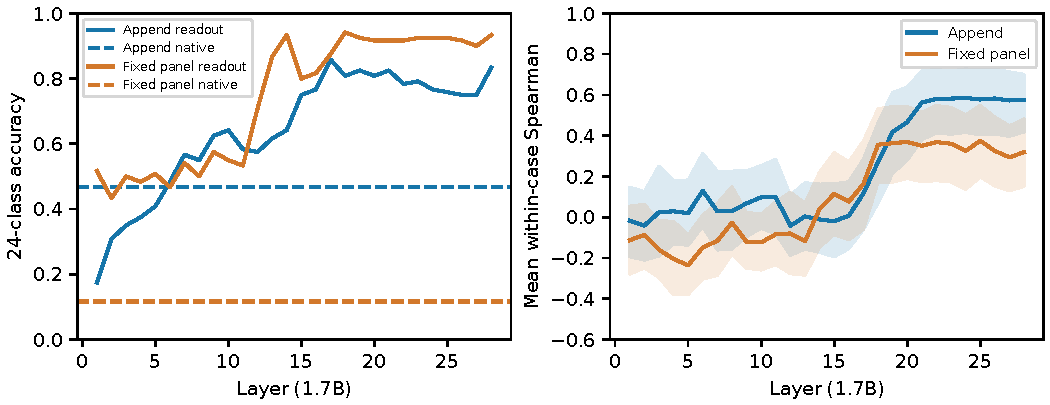
\includegraphics[width=.94\textwidth]{figures/depth_alignment.pdf}
\caption{Two different questions across depth. Left: independent-patient disease decoding versus native 24-class ranking (120 endpoints). Right: within-patient association between readout-margin and native-margin updates (24 trajectories); shaded bands are patient-bootstrap 95\% intervals. High endpoint decodability does not imply an equally strong relationship to output updating.}\label{fig:depth}
\end{figure*}

The discrepancy is not an aggregate illusion in which the two methods succeed on disjoint patients. Under append input, both are correct on 52 patients, only the readout on 48, only native ranking on four, and neither on 16. Under the panel, the corresponding counts are 13, 99, one, and seven. These four cells rule out both ``the internal readout is always right'' and ``the model ignores all disease information.'' They describe complementary observations, not access to a privileged internal ground truth.

\paragraph{Evidence-related internal changes remain connected to output.}
For each update, fix the pair consisting of the source disease $g$ and the strongest non-$g$ native competitor among the 24 classes at the previous round. We compare
\begin{align}
\Delta M_t &= \Delta[L_t(g)-L_t(c)],\\
\Delta S_{t,\ell} &= \Delta[s_{t,\ell}(g)-s_{t,\ell}(c)].
\end{align}
The competitor can change between events, but is fixed across the two prefixes of an event. We calculate Spearman correlation within each patient and average over patients.

At layer 28, mean correlation is 0.575 for append and 0.319 for the panel. The paired difference is $-0.256$ (95\% CI [$-0.446,-0.059$]). Nonzero changes point in the same direction on a patient-averaged 73.9\% and 62.6\% of updates. Thus internal and output changes are related, but presentation weakens their association. Figure~\ref{fig:depth} also separates endpoint decodability from the depth at which natural updates become more closely associated with output. These curves do not identify a unique causal layer.

Using only top-class changes would obscure this relationship. Among native 24-class switches, the layer-28 readout top remains unchanged at case-weighted rates of 58.2\% under append and 54.5\% under the panel. A readout can retain its top class while its margin moves with native output. We therefore interpret discrete disagreement together with continuous alignment, not as proof of independent internal and external beliefs.

\paragraph{Representation quality is source-dependent.}
A simple classifier trained on old patients reaches 120/120 on new full text; question-only text reaches 119/120 and recorded-field presence reaches 120/120. These controls show that the simulator's recording structure is highly predictive. A layer readout may exploit this structure rather than a disease concept abstracted from clinical reasoning. Keeping this baseline in the main argument prevents the decoding result from being misrepresented as discovering a superior clinical diagnostic method.

\section{RQ3: Can Internal Disease Information Change the Answer?}
\label{sec:causal}
\paragraph{Directional interventions.}
At the predetermined middle prefix for each of 24 patients and each presentation, take the source label $g$ and the strongest competing class $c$. Use the corresponding independently trained readout weights to define
\begin{align}
 v_\ell &= \frac{W_{\ell,:,g}-W_{\ell,:,c}}{\lVert W_{\ell,:,g}-W_{\ell,:,c}\rVert_2},\\
 h' &= h+\alpha\lVert h\rVert_2 v_\ell.
\end{align}
The primary dose is $\alpha=0.05$; 0.02 is an anchor sensitivity condition. We intervene at layers 21 and 28, either at the final prompt anchor or at all scored continuation positions. Controls use the opposite direction, a fixed orthogonal random direction of equal norm, and zero displacement. The source label is used as an offline intervention target, not as information available to a diagnostic system.

The independent outcome is the original model's target-versus-competitor log-score ratio. Increasing the external readout's own score would be a built-in consequence of the intervention and is not evidence of native use. There are 672 active conditions and 48 zero controls; every zero control reproduces its baseline.

\begin{figure*}[t]
\centering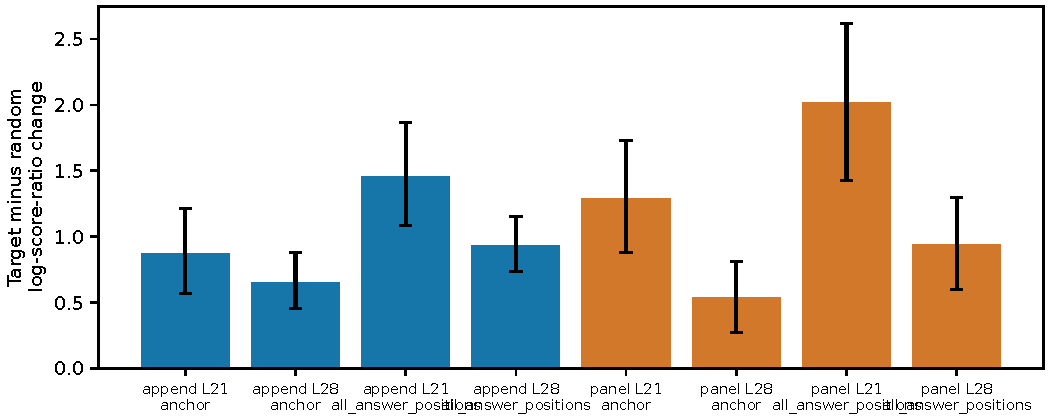
\includegraphics[width=.94\textwidth]{figures/causal.pdf}
\caption{Disease-direction effects on the original model's complete-name score ratio. All eight primary target-minus-random contrasts are positive after Holm correction ($p\leq0.00065$). Error bars are patient-bootstrap 95\% intervals. None of the eight target-direction conditions produces a newly correct top-49 diagnosis at dose 0.05.}\label{fig:causal}
\end{figure*}

\paragraph{Information has local causal influence.}
All eight primary target-minus-random comparisons are positive after Holm correction. Effects range from 0.539 to 2.017 log-score-ratio units (Figure~\ref{fig:causal}); opposite-direction mean effects are negative and the smaller anchor dose produces smaller mean effects. This establishes that these directions can influence the model's native scoring. It does not estimate how much of a natural evidence update is mediated by those directions, because an artificial displacement is not the same as removing the natural update.

\paragraph{Influence does not imply a corrected decision.}
No wrong-to-right or right-to-wrong top-49 transitions occur in the eight primary target conditions. For the layer-21 all-continuation intervention, append accuracy remains 10/24 and panel accuracy remains 5/24 at these middle prefixes. Among initially wrong cases, the median deficit of the source disease behind the strongest competing name is 10.681 log-score units for append and 22.119 for the panel. Median margin gains are only 1.166 and 1.516. The tested intervention therefore moves the score in the intended direction but usually leaves a much larger diagnostic deficit. This explains the observed local effect without presenting it as a successful correction method.

\paragraph{Where a state is changed determines what it can affect.}
For a causal decoder, changing the final-layer post-MLP state at the final prompt position alters the next-token logits but does not rewrite that layer's already computed key/value cache. Under fixed teacher-forced candidate continuations, only the first output-token score changes. Consequently, if two disease names share their first token,
\begin{equation}
 \Delta\{L(d_1)-L(d_2)\}=0.
\end{equation}
This is an architectural property of the intervention site, not a new theorem or a claim about all natural evidence updates.

The actual tokenizer groups medically different names: Panic attack, Pneumonia, Pulmonary embolism, and Pulmonary neoplasm share first token \texttt{P}; six Acute names share \texttt{Ac}. The layer-28 anchor intervention has exactly zero within-first-token selectivity. The layer-21 anchor has positive selectivity under append input (target-minus-random 0.134, CI [0.044,0.242], 13 applicable patients), while continuation interventions can influence later name tokens. Format-token effects are negligible in the measured decomposition. Disease-score movement must therefore be localized to its generation pathway before it is interpreted as changing a coherent disease belief.

\section{When Do the Three Levels Come Apart?}
\label{sec:conditions}
\paragraph{Patient answers matter, but do not uniquely determine choice.}
For each of 24 patients, we change one source-recorded binary Yes answer near the middle prefix to No, leaving its question and input length unchanged. Five cases change their top-49 disease; layer-21 and layer-28 readout tops change for seven and four. This establishes sensitivity to answer values in some cases. The counterfactual has no adjudicated new diagnosis, so we do not score its correctness. It also does not establish that unchanged answers imply semantic insensitivity. Negation sensitivity is a pre-existing evaluation problem \citep{negation}; here it is a control on the patient-specific interpretation.

\paragraph{Attention and diagnostic use can diverge.}
Placing known rows first or last in the panel preserves each patient's exact token count. Moving them last increases late-layer anchor attention to known facts from 2.05\% to 3.99\%, while source-label matches fall from 7/24 to 2/24. The paired accuracy permutation test yields $p=0.0634$, not a significant result at 0.05; the exploratory support difference is $-0.2185$ ($p=0.0070$, uncorrected). The observations show that greater attention mass does not establish improved evidence use. Attention mass is also affected by token grouping and is not a causal importance score.

Removing Unknown rows while retaining all known facts raises native accuracy from 3/24 to 12/24 relative to the original fixed panel. This implicates the presentation context, but the shortened condition changes both length and content and does not isolate a unique mechanism. Readouts trained on the original panel also degrade under these transformations; their cross-layout transfer cannot be assumed.

\paragraph{Default output preference explains only part of the failure.}
In age/sex-only prompts without symptoms, the 1.7B model selects COPD in all 24 cases both with and without the questionnaire. Mean support is 0.9990 and 0.9950 respectively. The questionnaire did not create the entire preference. With complete facts, reversing the candidate list reduces COPD selections from 17/24 to 2/24; rotating it reduces them to 8/24. The model never selects the new first candidate in these controls, ruling out a simple first-item copying rule.

Following the idea of content-free calibration \citep{calibrate}, we subtract each matched empty-input log score from its full-input score with fixed coefficient one. COPD selections disappear, but panel accuracy changes only from 3/24 to 5/24; append accuracy changes from 11/24 to 14/24. The paired gain intervals include zero. Removing a common answer preference does not automatically make the retained information determine the correct diagnosis. This is a diagnostic control, not a new calibration algorithm.

\paragraph{A second configuration improves accuracy, not invariance.}
The 4B configuration identifies 75/120 source labels natively among 49 diseases, compared with 44/120 for 1.7B. In the matched 24-class comparison, its last-layer readout still outperforms native ranking, 110/120 versus 82/120 (paired difference 23.3 points, CI [14.2,32.5]). Its final-layer natural-update correlation is 0.677, with 81.4\% same-direction updates. These results reinforce the distinction between increasing diagnostic competence and eliminating the information--decision discrepancy.

On the same 24 deep patients, 4B append input gives 16 correct endpoints, while the panel gives four (paired difference $-0.50$, CI [$-0.708,-0.292$]). Its most frequent panel answer is pulmonary embolism (10/24), rather than the 1.7B configuration's COPD concentration. Thus the presentation failure replicates, but the specific preferred disease does not. We did not repeat causal interventions in 4B or train 4B panel readouts.

\section{Related Work}
\paragraph{Belief revision and clinical updating.}
\citet{derelab} generate formally verified multi-turn defeasible reasoning tasks and study confirmation bias. Their turn-level truth permits normative revision judgments that our incomplete patient prefixes do not. \citet{zeng2026} study longitudinal clinical judgments and the influence of previous assessments. We exclude previous answers to isolate the mapping from cumulative facts to current computation. \citet{arun2026} evaluate stated diagnostic distributions on DDxPlus, including order, redundancy, and anchoring. Our primary distribution is calculated from model likelihoods of disease-name strings, and our focus is its relationship to layer states and interventions, not the first demonstration of clinical inconsistency.

\paragraph{Medical representations and causal intervention.}
\citet{marinescu2025} combine medical representation visualization, gradients, lesions, and patching, including nonmonotonic representations of disease progression. We study acquisition of evidence about a fixed patient rather than disease progression. Activation-direction steering is also established \citep{iti}. Our intervention contribution is the comparison between independent-patient directions, full-name output changes, and diagnostic boundary crossing, with explicit intervention-position controls.

\paragraph{Measurement of representations and answers.}
\citet{probing,contextprobe} motivate our separation of decodability from task use and the strong text baselines. Surface-form competition \citep{surface} motivates treating canonical-name support as a measurement interface rather than a disease posterior. Contextual calibration \citep{calibrate} motivates the empty-input score control. These methods inform the analysis; the contribution is the connected evidence about when medical information is preserved, updated, and expressed in a diagnostic choice.

\section{Conclusion}
Medical belief cannot be inferred from a confident diagnosis or a successful probe alone. In our experiments, patient evidence produces disease-related internal changes that correlate with native updates and admit directional causal influence. Yet the same information can coexist with incorrect, presentation-sensitive diagnosis, and a positive score intervention need not cross the diagnostic boundary. Exhaustive trajectories and counterexamples show that this relationship is conditional rather than a universal hidden-correct-answer phenomenon. The resulting account connects three measurable levels---disease information, evidence-driven updating, and diagnostic choice---and identifies the points where they cease to move together.

\section*{Limitations}
The study uses one synthetic generator, 120 held-out endpoints, and 24 deep trajectories spanning 17 diseases. Questions and recorded-field masks can predict labels, so readouts may exploit simulation structure. There are no ground-truth intermediate posteriors or adjudicated counterfactual diagnoses. The 49 canonical names constrain output, and string scores are not clinical probabilities. Both models are Qwen3 with explicit thinking disabled; size and quantization are confounded. Fixed heads receive supervision unavailable to native ranking. Causal interventions use known target labels and can move states off their natural distribution; they demonstrate local controllability, not natural causal mediation or a deployable diagnostic repair. Attention and residual decomposition are descriptive. Presentation follow-ups reuse observed patients, and the new trajectory taxonomy is post-hoc. Cross-family replication, matched-precision scaling, alternative case sources, and natural-update ablation remain substantive empirical extensions.

\section*{Ethics Statement}
We analyze language-model behavior on pre-existing synthetic cases, not new patient records or clinical interventions. Source diagnoses provide evaluation labels; this work adds no clinical adjudication. Results should not be interpreted as validation for patient care. Counterfactual answers are used to inspect computation and are not assigned invented disease labels. We retain source identifiers and distinguish acquired information from disease progression. The manuscript and analysis code were developed with an AI coding assistant; the research team remains responsible for their verification and final submission.

\bibliography{references}
\bibliographystyle{acl_natbib}
\clearpage
\appendix
\section{Reproducibility and Detailed Measurements}\label{app:repro}
\paragraph{Cohorts.} The 120 new patients comprise 30 respiratory, 20 cardiovascular, 20 digestive, 20 neurologic, 15 ear/nose/throat, and 15 systemic cases. Their 24 deep trajectories comprise 6, 2, 4, 6, 3, and 3 respectively, with 4--15 updates per case. Each disease has five endpoint patients, but the deep subset is not one case per disease. No exact fact-set overlap with prior cohorts was found, ignoring age and sex. This is an identity check, not a test for simulator-level overlap or pretraining contamination.

\paragraph{Counts.} The completed continuation produced 1,488 natural/input-control observations: 800 main 1.7B observations, 24 No-counterfactual observations, 120 presentation controls, 96 empty-input/candidate-order controls, and 448 4B observations. These include training measurements and repeated conditions; they are not independent patient counts. In addition there are 672 active intervention conditions and 48 zero controls. The present case synthesis adds no model calls. All inference was local, with zero API expenditure.

\paragraph{Architecture and runtime.} Qwen3-1.7B has 28 layers, hidden size 2048, 16 query heads, and eight key/value heads. The 4B configuration has 36 layers, hidden size 2560, 32 query heads, and eight key/value heads; its existing 8-bit quantization uses group size 128. Floating parameters use FP16. Model inference uses MLX on an Apple M2 Pro with 32 GB shared memory; statistical analyses use Python, NumPy, SciPy, and scikit-learn. Recorded manifests retain source and weight hashes. Greedy continuations and teacher-forced candidate scoring use the same evidence and candidate vocabulary. No model parameter is updated.

\paragraph{Readout objective.} Let $Z$ be the matrix of centered, normalized training states at one layer, and $Y$ the one-hot label matrix. We compute
\begin{equation}
 W=Z^\top(ZZ^\top+\lambda I)^{-1}(Y-\bar Y),
\end{equation}
with $b=\bar Y$ and $\lambda=0.1$. Heads are fitted separately for every layer. A separate head for each input presentation avoids silently treating cross-layout readout failure as missing information. Presentation follow-up readouts are evaluated with the original panel head and therefore measure transfer under a changed layout. Endpoint 4B final-layer accuracies at $\lambda=0.01,0.1,1$ are 92.5\%, 91.7\%, and 89.2\%. No test-prefix labels enter fitting.

\paragraph{Internal computation.} For each layer, we save residual input $h^{in}$, attention increment $a$, post-attention state $h^{attn}$, MLP increment $m$, and residual output $h^{out}$. We check $h^{attn}=h^{in}+a$ and $h^{out}=h^{attn}+m$, and continuity into the next layer. Projecting these additive terms through a fixed linear disease contrast decomposes the readout margin algebraically; it does not causally attribute medical reasoning to attention or MLP.

\paragraph{Attention.} The 1.7B endpoint atlas contains 107,520 patient--presentation--layer--head rows ($120\times2\times28\times16$). It measures the diagnostic anchor's attention toward known facts, unknown fields, candidates, and other prompt tokens. Layers 21--28 average known-fact mass is 4.23\% for append and 2.92\% for the original panel; candidate mass is 21.98\% and 15.44\%. The remaining mass includes instructions and formatting and must not be interpreted as medically irrelevant. Per-token-normalized masses are also retained. The full all-position attention tensor is not part of the current capture.

\paragraph{Exact instruction text.} The shared system instruction is:
\begin{quote}\small
You are analyzing a synthetic patient record for research. Compare the listed diagnoses using only the cumulative findings shown. Distinguish past medical history from the current presentation. Missing information is unknown. Some recorded ordinal scales have unspecified endpoint meanings; do not invent a clinical interpretation for their endpoints.
\end{quote}
The panel adds: ``Fixed questionnaire. Unknown means not available; it does not mean No.'' The common response instruction is:
\begin{quote}\small
Select the best-supported candidate for the current presentation at this point. Choose one listed diagnosis even if evidence is incomplete. Complete the JSON object with exactly one candidate diagnosis copied verbatim from the list. Do not abbreviate or add an explanation. The output must have the form \texttt{\{"diagnosis":"exact candidate diagnosis"\}}.
\end{quote}
The chat template uses \texttt{enable\_thinking=False}; the scored assistant prefix is \texttt{\{"diagnosis":"}. Append input includes source evidence-group identifiers; the panel uses the fixed question list. Known-field markers and identifiers are part of the measured presentation, so we do not assume purely semantic equivalence of the complete prompt strings.

\paragraph{Intervention sites and output scores.} Anchor interventions modify only the final prompt position. All-continuation interventions modify the same layer at each scored continuation position, including disease-name and formatting positions, with the local state norm determining displacement magnitude. Thus an all-continuation effect may act directly on disease-name generation, rather than on a single stored pre-answer belief. Character offsets split name and formatting tokens; tokens spanning a boundary count as name tokens. Both full-49 and sampled-24 competitor contrasts are retained. Same-first-token selectivity applies to 13/24 cases and is secondary.

\paragraph{Numerical checks.} All 48 intervention prefixes pass stability checks; none is excluded. Zero interventions preserve outputs exactly. Maximum relative RMS errors in attention reconstruction are $2.523\times10^{-4}$ (1.7B) and $2.480\times10^{-4}$ (4B). Maximum cached-versus-full sequence log-score errors are 0.01727 and 0.03084. These are implementation tolerances, not statistical error bars. Model weights are unchanged by hash before and after inference. All 120 presentation-control prompts were reconstructed with exact input-ID and token-group matches. A metadata discrepancy affecting the recorded baseline descriptor for append-with-24-candidates was documented; actual saved prompts and scores remain intact.

\paragraph{Analysis chronology.} Fixed-panel measurement and disease-direction experiments have frozen protocols and code snapshots. Answer-polarity, second-configuration, presentation, and empty-input controls were added sequentially to investigate observed discrepancies. Continuous update alignment and the exhaustive trajectory taxonomy are post-hoc analyses of existing records. Empty-input score subtraction was specified before those control observations were obtained. The protocols are project-local records, not a public preregistration. No follow-up is described as an independent new patient replication.

\section{Robustness and Scope of the Diagnostic Interface}
\label{app:robust}
\paragraph{Output parsing and string mass.} For 1.7B, the median probability mass of the scored canonical strings is 0.99279 in append and 0.98875 in the panel; 14/120 and 1/120 cases respectively have mass below 0.1. Greedy diagnostic matches are 38/120 and 10/120, versus sequence-ranked 44/120 and 10/120. The native presentation gap therefore also appears in greedy continuations. Sequence-sum and mean-token top choices agree in 90\% and 95\% of cases. For 4B append, greedy matches are 75/120, 117/120 continuations are canonical candidates, median mass is 0.999943, and 119/120 sequence/mean-token top choices agree.

\paragraph{Candidate sets.} The primary 24-class ranking is computed inside a 49-candidate prompt. On the 24 deep cases, changing the prompt itself to 24 candidates gives 6/24 correct panel endpoints and 15/24 append endpoints; reranking the 49-name prompt over those classes gives 4/24 and 12/24. These paired gains have intervals spanning zero and do not remove supervision differences with the probes.

\paragraph{Reference agreement.} Restricting to the 79 cases where the pathology label is also top in the reference differential gives native/readout24 counts of 42/67 for append and 10/77 for the panel, all with denominator 79. This rules out label--differential disagreement as the sole explanation of the observed discrepancy. It does not supply missing intermediate clinical truth.

\paragraph{Disease groups.} Table~\ref{tab:families} shows that the aggregate effect does not require every group to improve internally. Group estimates are descriptive; only five patients represent each disease.
\begin{table}[h]
\centering\small
\begin{tabular}{lrrr}\toprule
Group ($n$) & Native A/P & Probe A/P\\\midrule
Respiratory (30) & 12/9 & 25/28\\
Cardiovascular (20) & 4/1 & 13/19\\
Digestive (20) & 10/0 & 15/20\\
Neurologic (20) & 17/0 & 20/19\\
ENT (15) & 9/0 & 13/15\\
Systemic (15) & 4/4 & 14/11\\\bottomrule
\end{tabular}
\caption{Counts correct in append/panel, same 24 diseases. Probe refers to layer 28.}\label{tab:families}
\end{table}

\paragraph{Input-value controls.} A presence-only representation that hides answer values while retaining known-field positions gives 0/24 native correct diagnoses in the tested panel control. This does not conflict with a supervised field-presence classifier reaching 120/120 on endpoints: the classifier is explicitly trained to exploit the recording pattern, whereas the original model is not. The comparison reinforces the distinction between available predictive information and native use.

\paragraph{Unresolved experiments.} The existing causal test shows a directional effect, not necessity of a natural update. A stronger test would remove the projection of an actual adjacent-prefix state difference onto a direction fixed using different patients and compare same-norm random removal, old-state replacement, and self replacement. A new cohort should confirm layer and dose choices. Other priorities are evidence-pattern-matched cross-diagnosis cases, alternative case sources, precision-matched models, and explicit-thinking conditions. These experiments are not reported as completed.

\section{Ten Contrasting Examples}\label{app:examples}
The following gallery deliberately spans different trajectories; it is illustrative and was selected after analysis. Population counts always include the full 24 preselected patients. The source label supplies a common coordinate for plotting support; it does not prescribe a correct posterior at every partial prefix.

\begin{enumerate}
\item \textbf{Otitis media, 0041136}: the treatment-history group moves append output to the label, which remains selected; the panel keeps COPD despite readable otitis information.
\item \textbf{Pancreatic neoplasm, 0027885}: append output enters the label twice and ultimately selects bronchiolitis, while the endpoint readout selects pancreatic neoplasm.
\item \textbf{Acute dystonic reactions, 0032489}: the append output remains acute laryngitis throughout; the endpoint readout selects the label. This is persistent error without diagnostic oscillation.
\item \textbf{Boerhaave, 0044249}: append output recovers the label at the endpoint, while the final readout selects GERD. This directly challenges the idea of an always-correct hidden answer.
\item \textbf{Pulmonary embolism, 0048692}: append output ends at acute pulmonary edema and the readout at spontaneous pneumothorax. Both channels fail.
\item \textbf{Anemia, 0006854}: append output enters anemia and later returns to pulmonary embolism; the panel ends at anemia. This is a counterexample to uniform panel harm.
\item \textbf{Spontaneous pneumothorax, 0101113}: both append and panel end at the label. Different presentations can converge successfully.
\item \textbf{Guillain--Barr\'{e} syndrome, 0079685}: append output visits several alternatives before eventually reaching the source label. This illustrates delayed acquisition rather than a stable correct diagnosis from the first evidence.
\item \textbf{Pericarditis, 0037913}: append output enters pericarditis, later moves to laryngitis, and ends at Boerhaave, while the final readout selects pericarditis.
\item \textbf{GERD, 0123136}: append output shifts from pulmonary edema to the source label and retains it; panel output ends at COPD. This repeats presentation-dependent separation outside the opening ENT example.
\end{enumerate}
\begin{figure*}[p]
\centering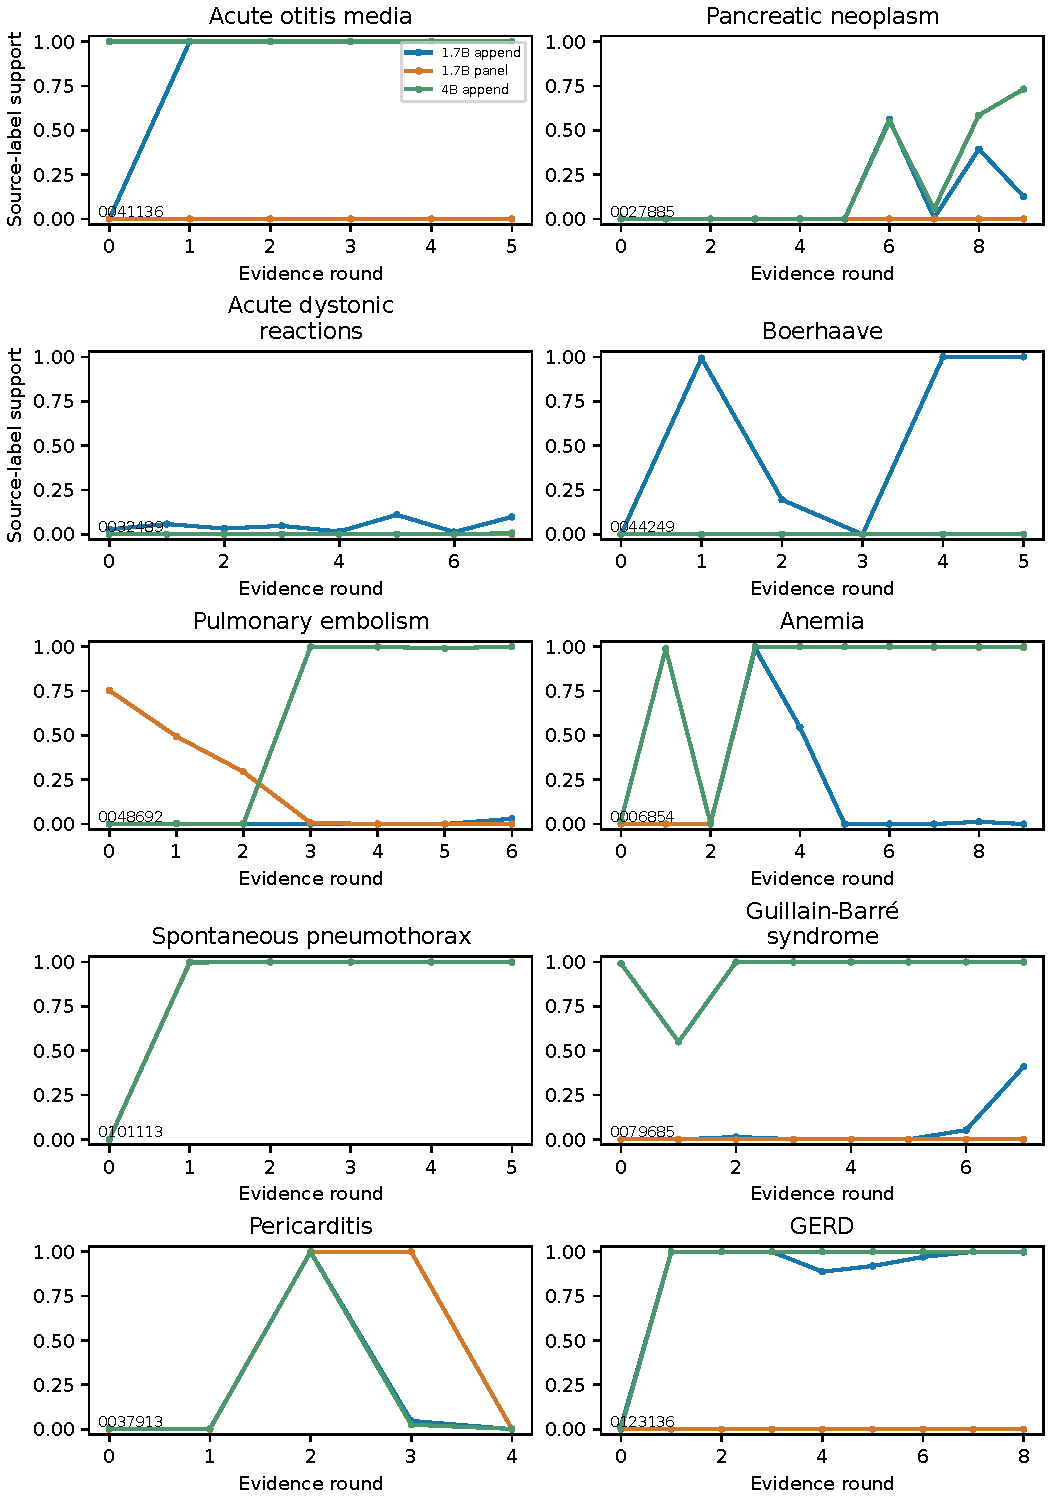
\includegraphics[width=.94\textwidth,height=.84\textheight,keepaspectratio]{figures/case_gallery.pdf}
\caption{Ten contrasting patients. Each line is the model-native relative support for the patient's source-label disease, not a probe probability. Blue: 1.7B append; orange: 1.7B panel; green: 4B append. Source evidence and competing disease identities for every round are given in the complete case appendix.}
\end{figure*}

\clearpage\onecolumn
\section{Complete Patient Evidence and Trajectories}\label{app:cases}
All 24 preselected patients are included. Native supports are normalized over 49 names. Readout tops are predictions of separate 24-class heads trained on old-patient endpoints; their labels are not model-native probabilities. The figures show source-label support and maximal native support above, and the source label's rank in every layer readout below (yellow is rank 1). Tables give each newly available evidence group and the full top-disease trajectory in three conditions. The companion repository contains every candidate score and all-layer heatmaps.
\subsection{ddx\_test\_0005881 -- Anemia}
\label{case:ddx_test_0005881}

Source label: Anemia. Family: systemic. Evidence updates: 15. All facts below are source-recorded; their order is acquisition order.

\begin{center}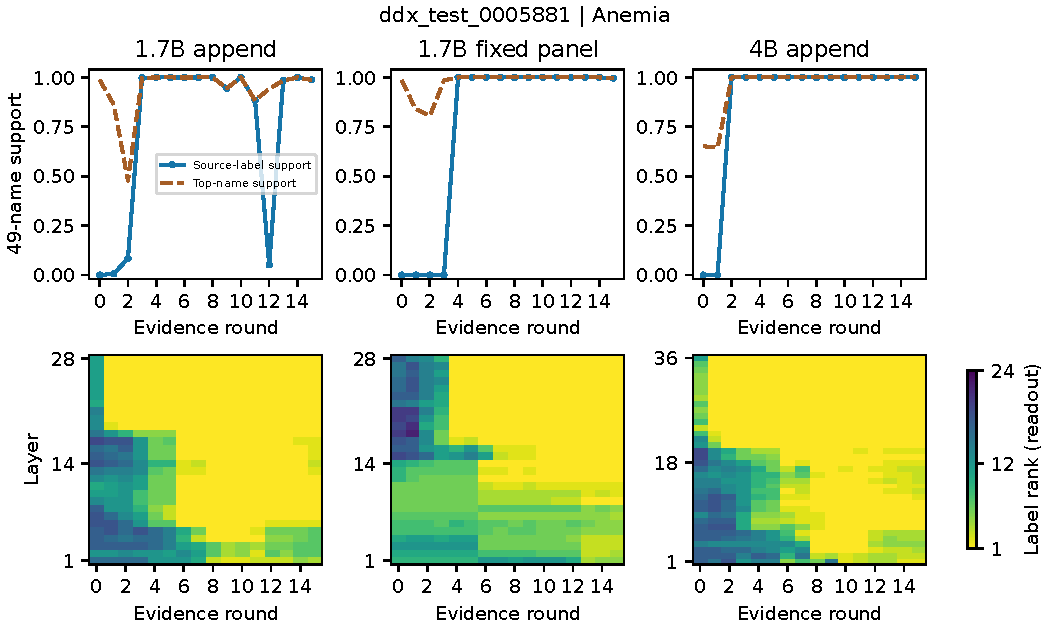
\includegraphics[width=.96\linewidth]{figures/ddx_test_0005881.pdf}\end{center}

{\small\begin{longtable}{>{\raggedright\arraybackslash}p{.07\textwidth}>{\raggedright\arraybackslash}p{.415\textwidth}>{\raggedright\arraybackslash}p{.415\textwidth}}\toprule Round & Newly revealed source evidence & Native top / label support / final-layer probe top \\ \midrule\endhead

0 & Are you experiencing shortness of breath or difficulty breathing in a significant way? Yes & 1.7B append: Acute COPD exacerbation / infection / 0.0000 / Bronchitis\newline 1.7B panel: Acute pulmonary edema / 0.0000 / Guillain-Barr\'{e} syndrome\newline 4B append: Acute rhinosinusitis / 0.0000 / Bronchitis \\ 

1 & Have you recently had stools that were black (like coal)? Yes & 1.7B append: Acute COPD exacerbation / infection / 0.0065 / Anemia\newline 1.7B panel: Acute pulmonary edema / 0.0000 / Guillain-Barr\'{e} syndrome\newline 4B append: Pulmonary embolism / 0.0006 / Anemia \\ 

2 & Is your BMI less than 18.5, or are you underweight? Yes & 1.7B append: Acute COPD exacerbation / infection / 0.0840 / Anemia\newline 1.7B panel: Acute pulmonary edema / 0.0000 / Guillain-Barr\'{e} syndrome\newline 4B append: Anemia / 0.9999 / Anemia \\ 

3 & Do you have any family members who have been diagnosed with anemia? Yes & 1.7B append: Anemia / 0.9983 / Anemia\newline 1.7B panel: Acute pulmonary edema / 0.0000 / Guillain-Barr\'{e} syndrome\newline 4B append: Anemia / 1.0000 / Anemia \\ 

4 & Have you ever had a diagnosis of anemia? Yes & 1.7B append: Anemia / 0.9998 / Anemia\newline 1.7B panel: Anemia / 1.0000 / Anemia\newline 4B append: Anemia / 1.0000 / Anemia \\ 

5 & Do you feel so tired that you are unable to do your usual activities or are you stuck in your bed all day long? Yes & 1.7B append: Anemia / 1.0000 / Anemia\newline 1.7B panel: Anemia / 1.0000 / Anemia\newline 4B append: Anemia / 1.0000 / Anemia \\ 

6 & Do you have pain somewhere, related to your reason for consulting? Yes; Characterize your pain: sensitive; tugging; exhausting; Do you feel pain somewhere? back of head; top of the head; forehead; How intense is the pain? Recorded scale value 3 on the dataset's 0-10 scale; endpoint meanings are unspecified; Does the pain radiate to another location? nowhere; How precisely is the pain located? Recorded scale value 5 on the dataset's 0-10 scale; endpoint meanings are unspecified; How fast did the pain appear? Recorded scale value 4 on the dataset's 0-10 scale; endpoint meanings are unspecified & 1.7B append: Anemia / 0.9992 / Anemia\newline 1.7B panel: Anemia / 1.0000 / Anemia\newline 4B append: Anemia / 1.0000 / Anemia \\ 

7 & Do you have chronic kidney failure? Yes & 1.7B append: Anemia / 0.9999 / Anemia\newline 1.7B panel: Anemia / 1.0000 / Anemia\newline 4B append: Anemia / 1.0000 / Anemia \\ 

8 & Do you think you are pregnant or are you currently pregnant? Yes & 1.7B append: Anemia / 1.0000 / Anemia\newline 1.7B panel: Anemia / 1.0000 / Anemia\newline 4B append: Anemia / 1.0000 / Anemia \\ 

9 & Do you feel slightly dizzy or lightheaded? Yes & 1.7B append: Anemia / 0.9450 / Anemia\newline 1.7B panel: Anemia / 1.0000 / Anemia\newline 4B append: Anemia / 1.0000 / Anemia \\ 

10 & Are you taking any new oral anticoagulants ((NOACs)? Yes & 1.7B append: Anemia / 1.0000 / Anemia\newline 1.7B panel: Anemia / 1.0000 / Anemia\newline 4B append: Anemia / 1.0000 / Anemia \\ 

11 & Do you have very abundant or very long menstruation periods? Yes & 1.7B append: Anemia / 0.8839 / Anemia\newline 1.7B panel: Anemia / 1.0000 / Anemia\newline 4B append: Anemia / 1.0000 / Anemia \\ 

12 & Do you feel lightheaded and dizzy or do you feel like you are about to faint? Yes & 1.7B append: Acute pulmonary edema / 0.0515 / Anemia\newline 1.7B panel: Anemia / 1.0000 / Anemia\newline 4B append: Anemia / 1.0000 / Anemia \\ 

13 & Have you traveled out of the country in the last 4 weeks? Central America & 1.7B append: Anemia / 0.9843 / Anemia\newline 1.7B panel: Anemia / 1.0000 / Anemia\newline 4B append: Anemia / 1.0000 / Anemia \\ 

14 & Do you constantly feel fatigued or do you have non-restful sleep? Yes & 1.7B append: Anemia / 0.9996 / Anemia\newline 1.7B panel: Anemia / 1.0000 / Anemia\newline 4B append: Anemia / 1.0000 / Anemia \\ 

15 & Do you have a poor diet? Yes & 1.7B append: Anemia / 0.9875 / Anemia\newline 1.7B panel: Anemia / 0.9959 / Anemia\newline 4B append: Anemia / 1.0000 / Anemia \\ 

\bottomrule\end{longtable}}

\clearpage\subsection{ddx\_test\_0006854 -- Anemia}
\label{case:ddx_test_0006854}

Source label: Anemia. Family: systemic. Evidence updates: 9. All facts below are source-recorded; their order is acquisition order.

\begin{center}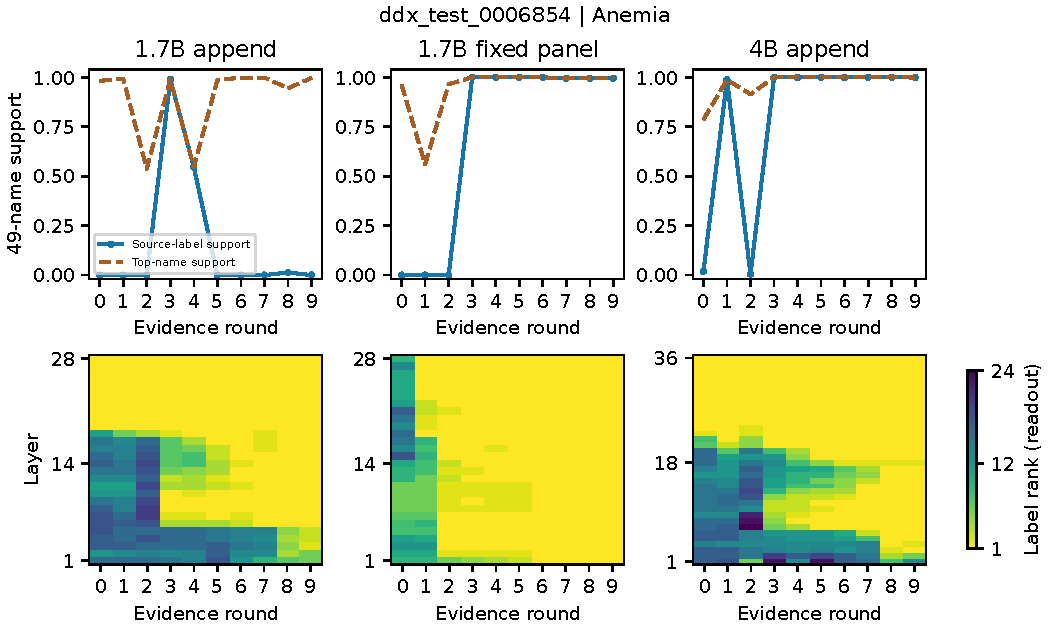
\includegraphics[width=.96\linewidth]{figures/ddx_test_0006854.pdf}\end{center}

{\small\begin{longtable}{>{\raggedright\arraybackslash}p{.07\textwidth}>{\raggedright\arraybackslash}p{.415\textwidth}>{\raggedright\arraybackslash}p{.415\textwidth}}\toprule Round & Newly revealed source evidence & Native top / label support / final-layer probe top \\ \midrule\endhead

0 & Have you noticed light red blood or blood clots in your stool? Yes & 1.7B append: Pulmonary embolism / 0.0000 / Anemia\newline 1.7B panel: Acute COPD exacerbation / infection / 0.0000 / HIV (initial infection)\newline 4B append: Pulmonary embolism / 0.0191 / Anemia \\ 

1 & Do you have chronic kidney failure? Yes & 1.7B append: Pulmonary embolism / 0.0000 / Anemia\newline 1.7B panel: Acute pulmonary edema / 0.0000 / Anemia\newline 4B append: Anemia / 0.9881 / Anemia \\ 

2 & Do you have pain somewhere, related to your reason for consulting? Yes; Characterize your pain: sensitive; a cramp; Do you feel pain somewhere? back of head; temple(R); How intense is the pain? Recorded scale value 5 on the dataset's 0-10 scale; endpoint meanings are unspecified; Does the pain radiate to another location? nowhere; How precisely is the pain located? Recorded scale value 8 on the dataset's 0-10 scale; endpoint meanings are unspecified; How fast did the pain appear? Recorded scale value 4 on the dataset's 0-10 scale; endpoint meanings are unspecified & 1.7B append: Pulmonary embolism / 0.0000 / Anemia\newline 1.7B panel: Acute COPD exacerbation / infection / 0.0000 / Anemia\newline 4B append: Pulmonary embolism / 0.0041 / Anemia \\ 

3 & Have you ever had a diagnosis of anemia? Yes & 1.7B append: Anemia / 0.9896 / Anemia\newline 1.7B panel: Anemia / 1.0000 / Anemia\newline 4B append: Anemia / 1.0000 / Anemia \\ 

4 & Is your BMI less than 18.5, or are you underweight? Yes & 1.7B append: Anemia / 0.5457 / Anemia\newline 1.7B panel: Anemia / 1.0000 / Anemia\newline 4B append: Anemia / 1.0000 / Anemia \\ 

5 & Have you recently had stools that were black (like coal)? Yes & 1.7B append: Pulmonary embolism / 0.0000 / Anemia\newline 1.7B panel: Anemia / 1.0000 / Anemia\newline 4B append: Anemia / 1.0000 / Anemia \\ 

6 & Have you traveled out of the country in the last 4 weeks? South Africa & 1.7B append: Pulmonary embolism / 0.0000 / Anemia\newline 1.7B panel: Anemia / 1.0000 / Anemia\newline 4B append: Anemia / 1.0000 / Anemia \\ 

7 & Do you have a poor diet? Yes & 1.7B append: Pulmonary embolism / 0.0000 / Anemia\newline 1.7B panel: Anemia / 0.9957 / Anemia\newline 4B append: Anemia / 1.0000 / Anemia \\ 

8 & Do you have any family members who have been diagnosed with anemia? Yes & 1.7B append: Pulmonary embolism / 0.0129 / Anemia\newline 1.7B panel: Anemia / 0.9957 / Anemia\newline 4B append: Anemia / 1.0000 / Anemia \\ 

9 & Are you taking any new oral anticoagulants ((NOACs)? Yes & 1.7B append: Pulmonary embolism / 0.0000 / Anemia\newline 1.7B panel: Anemia / 0.9957 / Anemia\newline 4B append: Anemia / 0.9997 / Anemia \\ 

\bottomrule\end{longtable}}

\clearpage\subsection{ddx\_test\_0017896 -- HIV (initial infection)}
\label{case:ddx_test_0017896}

Source label: HIV (initial infection). Family: systemic. Evidence updates: 11. All facts below are source-recorded; their order is acquisition order.

\begin{center}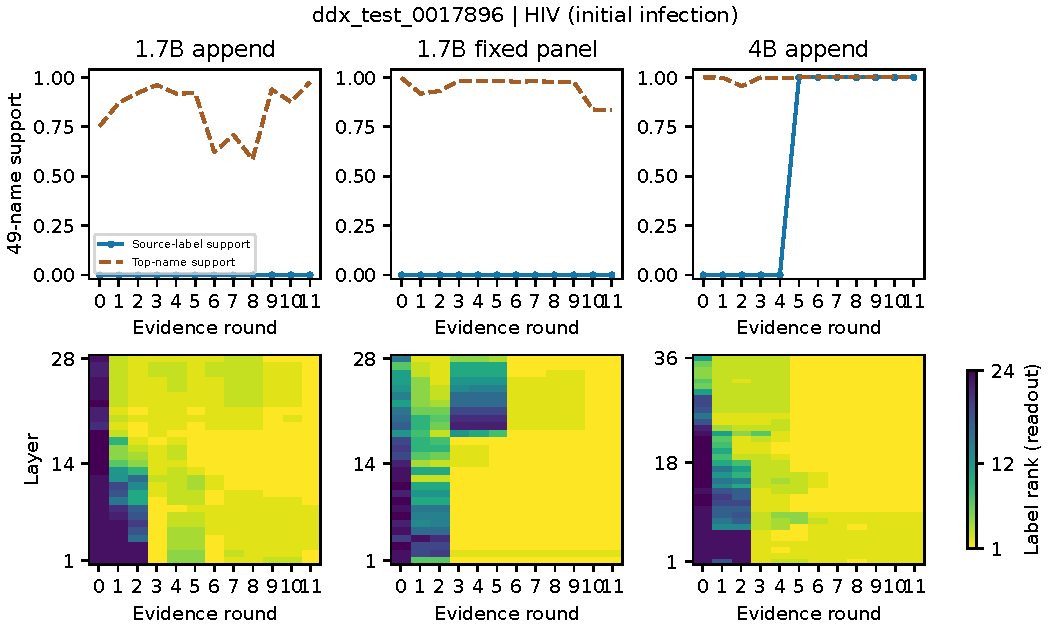
\includegraphics[width=.96\linewidth]{figures/ddx_test_0017896.pdf}\end{center}

{\small\begin{longtable}{>{\raggedright\arraybackslash}p{.07\textwidth}>{\raggedright\arraybackslash}p{.415\textwidth}>{\raggedright\arraybackslash}p{.415\textwidth}}\toprule Round & Newly revealed source evidence & Native top / label support / final-layer probe top \\ \midrule\endhead

0 & Do you have a sore throat? Yes & 1.7B append: Acute rhinosinusitis / 0.0000 / URTI\newline 1.7B panel: Acute COPD exacerbation / infection / 0.0000 / URTI\newline 4B append: Viral pharyngitis / 0.0000 / Viral pharyngitis \\ 

1 & Do you have any lesions, redness or problems on your skin that you believe are related to the condition you are consulting for? Yes; What color is the rash? pale; Do your lesions peel off? No; Is the rash swollen? Recorded scale value 2 on the dataset's 0-10 scale; endpoint meanings are unspecified; Where is the affected region located? lower gum; upper gum; internal cheek(R); internal cheek(L); bottom lip(R); How intense is the pain caused by the rash? Recorded scale value 5 on the dataset's 0-10 scale; endpoint meanings are unspecified; Is the lesion (or are the lesions) larger than 1cm? Yes; How severe is the itching? Recorded scale value 0 on the dataset's 0-10 scale; endpoint meanings are unspecified & 1.7B append: Viral pharyngitis / 0.0000 / URTI\newline 1.7B panel: Acute COPD exacerbation / infection / 0.0000 / URTI\newline 4B append: Viral pharyngitis / 0.0000 / Viral pharyngitis \\ 

2 & Have you had an involuntary weight loss over the last 3 months? Yes & 1.7B append: Acute rhinosinusitis / 0.0000 / URTI\newline 1.7B panel: Acute COPD exacerbation / infection / 0.0000 / URTI\newline 4B append: Viral pharyngitis / 0.0000 / SLE \\ 

3 & Do you have pain somewhere, related to your reason for consulting? Yes; Characterize your pain: tedious; sensitive; exhausting; Do you feel pain somewhere? back of head; top of the head; forehead; occiput; temple(L); How intense is the pain? Recorded scale value 6 on the dataset's 0-10 scale; endpoint meanings are unspecified; Does the pain radiate to another location? nowhere; How precisely is the pain located? Recorded scale value 8 on the dataset's 0-10 scale; endpoint meanings are unspecified; How fast did the pain appear? Recorded scale value 4 on the dataset's 0-10 scale; endpoint meanings are unspecified & 1.7B append: Acute rhinosinusitis / 0.0000 / URTI\newline 1.7B panel: Acute COPD exacerbation / infection / 0.0000 / SLE\newline 4B append: Viral pharyngitis / 0.0000 / Viral pharyngitis \\ 

4 & Have you had unprotected sex with more than one partner in the last 6 months? Yes & 1.7B append: Acute rhinosinusitis / 0.0000 / URTI\newline 1.7B panel: Acute COPD exacerbation / infection / 0.0000 / SLE\newline 4B append: Viral pharyngitis / 0.0000 / Viral pharyngitis \\ 

5 & Have you had sexual intercourse with an HIV-positive partner in the past 12 months? Yes & 1.7B append: Acute rhinosinusitis / 0.0000 / URTI\newline 1.7B panel: Acute COPD exacerbation / infection / 0.0000 / SLE\newline 4B append: HIV (initial infection) / 1.0000 / HIV (initial infection) \\ 

6 & Have you had significantly increased sweating? Yes & 1.7B append: Acute rhinosinusitis / 0.0000 / URTI\newline 1.7B panel: Acute COPD exacerbation / infection / 0.0000 / HIV (initial infection)\newline 4B append: HIV (initial infection) / 1.0000 / HIV (initial infection) \\ 

7 & Do you have diffuse (widespread) muscle pain? Yes & 1.7B append: Acute rhinosinusitis / 0.0000 / URTI\newline 1.7B panel: Acute COPD exacerbation / infection / 0.0000 / HIV (initial infection)\newline 4B append: HIV (initial infection) / 1.0000 / HIV (initial infection) \\ 

8 & Are you currently using intravenous drugs? Yes & 1.7B append: Acute rhinosinusitis / 0.0000 / URTI\newline 1.7B panel: Acute COPD exacerbation / infection / 0.0000 / HIV (initial infection)\newline 4B append: HIV (initial infection) / 1.0000 / HIV (initial infection) \\ 

9 & Have you traveled out of the country in the last 4 weeks? No & 1.7B append: Acute rhinosinusitis / 0.0000 / HIV (initial infection)\newline 1.7B panel: Acute COPD exacerbation / infection / 0.0000 / HIV (initial infection)\newline 4B append: HIV (initial infection) / 1.0000 / HIV (initial infection) \\ 

10 & Do you have swollen or painful lymph nodes? Yes & 1.7B append: Acute rhinosinusitis / 0.0000 / HIV (initial infection)\newline 1.7B panel: Acute COPD exacerbation / infection / 0.0000 / HIV (initial infection)\newline 4B append: HIV (initial infection) / 1.0000 / HIV (initial infection) \\ 

11 & Do you have a fever (either felt or measured with a thermometer)? Yes & 1.7B append: Acute rhinosinusitis / 0.0000 / HIV (initial infection)\newline 1.7B panel: Acute COPD exacerbation / infection / 0.0000 / HIV (initial infection)\newline 4B append: HIV (initial infection) / 1.0000 / HIV (initial infection) \\ 

\bottomrule\end{longtable}}

\clearpage\subsection{ddx\_test\_0027885 -- Pancreatic neoplasm}
\label{case:ddx_test_0027885}

Source label: Pancreatic neoplasm. Family: digestive. Evidence updates: 9. All facts below are source-recorded; their order is acquisition order.

\begin{center}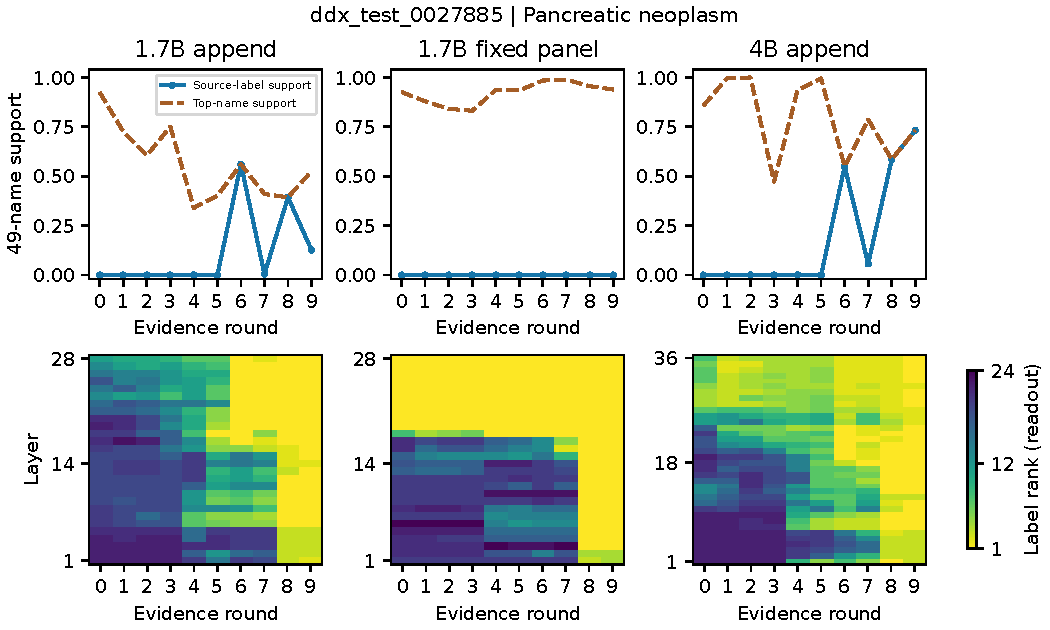
\includegraphics[width=.96\linewidth]{figures/ddx_test_0027885.pdf}\end{center}

{\small\begin{longtable}{>{\raggedright\arraybackslash}p{.07\textwidth}>{\raggedright\arraybackslash}p{.415\textwidth}>{\raggedright\arraybackslash}p{.415\textwidth}}\toprule Round & Newly revealed source evidence & Native top / label support / final-layer probe top \\ \midrule\endhead

0 & Have you had diarrhea or an increase in stool frequency? Yes & 1.7B append: Acute COPD exacerbation / infection / 0.0000 / Bronchitis\newline 1.7B panel: Acute COPD exacerbation / infection / 0.0000 / Pancreatic neoplasm\newline 4B append: Acute rhinosinusitis / 0.0000 / URTI \\ 

1 & Do you have diabetes? Yes & 1.7B append: Acute COPD exacerbation / infection / 0.0000 / Bronchitis\newline 1.7B panel: Acute COPD exacerbation / infection / 0.0000 / Pancreatic neoplasm\newline 4B append: Influenza / 0.0000 / URTI \\ 

2 & Have you traveled out of the country in the last 4 weeks? No & 1.7B append: Acute COPD exacerbation / infection / 0.0000 / HIV (initial infection)\newline 1.7B panel: Acute COPD exacerbation / infection / 0.0000 / Pancreatic neoplasm\newline 4B append: Influenza / 0.0000 / URTI \\ 

3 & Are you significantly overweight compared to people of the same height as you? Yes & 1.7B append: Acute COPD exacerbation / infection / 0.0000 / Anemia\newline 1.7B panel: Acute COPD exacerbation / infection / 0.0000 / Pancreatic neoplasm\newline 4B append: Influenza / 0.0000 / URTI \\ 

4 & Do you have pain somewhere, related to your reason for consulting? Yes; Characterize your pain: a cramp; Do you feel pain somewhere? flank(L); epigastric; How intense is the pain? Recorded scale value 1 on the dataset's 0-10 scale; endpoint meanings are unspecified; Does the pain radiate to another location? nowhere; How precisely is the pain located? Recorded scale value 1 on the dataset's 0-10 scale; endpoint meanings are unspecified; How fast did the pain appear? Recorded scale value 5 on the dataset's 0-10 scale; endpoint meanings are unspecified & 1.7B append: Acute rhinosinusitis / 0.0006 / Inguinal hernia\newline 1.7B panel: Acute COPD exacerbation / infection / 0.0000 / Pancreatic neoplasm\newline 4B append: Bronchitis / 0.0008 / Boerhaave \\ 

5 & Do you smoke cigarettes? Yes & 1.7B append: Acute rhinosinusitis / 0.0001 / Inguinal hernia\newline 1.7B panel: Acute COPD exacerbation / infection / 0.0000 / Pancreatic neoplasm\newline 4B append: Bronchitis / 0.0000 / Boerhaave \\ 

6 & Do you have chronic pancreatitis? Yes & 1.7B append: Pancreatic neoplasm / 0.5602 / Pancreatic neoplasm\newline 1.7B panel: Acute COPD exacerbation / infection / 0.0000 / Pancreatic neoplasm\newline 4B append: Pancreatic neoplasm / 0.5491 / Boerhaave \\ 

7 & Do you have a cough? Yes & 1.7B append: Acute rhinosinusitis / 0.0052 / Inguinal hernia\newline 1.7B panel: Acute COPD exacerbation / infection / 0.0000 / Pancreatic neoplasm\newline 4B append: Bronchitis / 0.0570 / Boerhaave \\ 

8 & Do you have any lesions, redness or problems on your skin that you believe are related to the condition you are consulting for? Yes; What color is the rash? yellow; Do your lesions peel off? No; Is the rash swollen? Recorded scale value 0 on the dataset's 0-10 scale; endpoint meanings are unspecified; Where is the affected region located? epigastric; How intense is the pain caused by the rash? Recorded scale value 2 on the dataset's 0-10 scale; endpoint meanings are unspecified; Is the lesion (or are the lesions) larger than 1cm? Yes; How severe is the itching? Recorded scale value 3 on the dataset's 0-10 scale; endpoint meanings are unspecified & 1.7B append: Pancreatic neoplasm / 0.3933 / Pancreatic neoplasm\newline 1.7B panel: Acute COPD exacerbation / infection / 0.0000 / Pancreatic neoplasm\newline 4B append: Pancreatic neoplasm / 0.5849 / Boerhaave \\ 

9 & Have you had an involuntary weight loss over the last 3 months? Yes & 1.7B append: Bronchiolitis / 0.1266 / Pancreatic neoplasm\newline 1.7B panel: Acute COPD exacerbation / infection / 0.0000 / Pancreatic neoplasm\newline 4B append: Pancreatic neoplasm / 0.7317 / Pancreatic neoplasm \\ 

\bottomrule\end{longtable}}

\clearpage\subsection{ddx\_test\_0032489 -- Acute dystonic reactions}
\label{case:ddx_test_0032489}

Source label: Acute dystonic reactions. Family: neurologic. Evidence updates: 7. All facts below are source-recorded; their order is acquisition order.

\begin{center}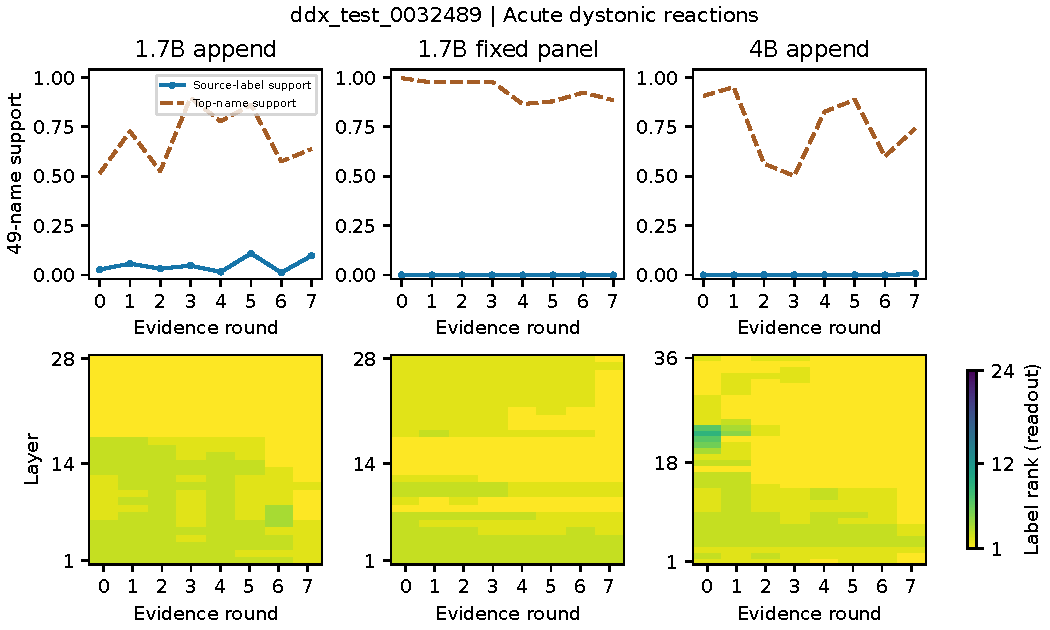
\includegraphics[width=.96\linewidth]{figures/ddx_test_0032489.pdf}\end{center}

{\small\begin{longtable}{>{\raggedright\arraybackslash}p{.07\textwidth}>{\raggedright\arraybackslash}p{.415\textwidth}>{\raggedright\arraybackslash}p{.415\textwidth}}\toprule Round & Newly revealed source evidence & Native top / label support / final-layer probe top \\ \midrule\endhead

0 & Do you feel that muscle spasms or soreness in your neck are keeping you from turning your head to one side? Yes & 1.7B append: Acute laryngitis / 0.0277 / Acute dystonic reactions\newline 1.7B panel: Acute COPD exacerbation / infection / 0.0001 / Myasthenia gravis\newline 4B append: Acute otitis media / 0.0000 / URTI \\ 

1 & Do you have a hard time opening/raising one or both eyelids? Yes & 1.7B append: Acute laryngitis / 0.0579 / Acute dystonic reactions\newline 1.7B panel: Acute COPD exacerbation / infection / 0.0000 / Myasthenia gravis\newline 4B append: Acute otitis media / 0.0000 / Acute dystonic reactions \\ 

2 & Do you regularly take stimulant drugs? Yes & 1.7B append: Acute laryngitis / 0.0326 / Acute dystonic reactions\newline 1.7B panel: Acute COPD exacerbation / infection / 0.0001 / Myasthenia gravis\newline 4B append: Acute laryngitis / 0.0013 / Myasthenia gravis \\ 

3 & Do you suddenly have difficulty or an inability to open your mouth or have jaw pain when opening it? Yes & 1.7B append: Acute laryngitis / 0.0475 / Acute dystonic reactions\newline 1.7B panel: Acute COPD exacerbation / infection / 0.0001 / Myasthenia gravis\newline 4B append: Acute laryngitis / 0.0009 / Myasthenia gravis \\ 

4 & Have you ever felt like you were suffocating for a very short time associated with inability to breathe or speak? Yes & 1.7B append: Acute laryngitis / 0.0159 / Acute dystonic reactions\newline 1.7B panel: Acute COPD exacerbation / infection / 0.0001 / Myasthenia gravis\newline 4B append: Panic attack / 0.0000 / Acute dystonic reactions \\ 

5 & Do you have trouble keeping your tongue in your mouth? Yes & 1.7B append: Acute laryngitis / 0.1095 / Acute dystonic reactions\newline 1.7B panel: Acute COPD exacerbation / infection / 0.0001 / Myasthenia gravis\newline 4B append: Panic attack / 0.0004 / Acute dystonic reactions \\ 

6 & Have you traveled out of the country in the last 4 weeks? No & 1.7B append: Acute laryngitis / 0.0127 / Acute dystonic reactions\newline 1.7B panel: Acute COPD exacerbation / infection / 0.0001 / Myasthenia gravis\newline 4B append: Panic attack / 0.0000 / Acute dystonic reactions \\ 

7 & Have you been treated in hospital recently for nausea, agitation, intoxication or aggressive behavior and received medication via an intravenous or intramuscular route? Yes & 1.7B append: Acute laryngitis / 0.0977 / Acute dystonic reactions\newline 1.7B panel: Acute COPD exacerbation / infection / 0.0000 / Acute dystonic reactions\newline 4B append: Panic attack / 0.0068 / Acute dystonic reactions \\ 

\bottomrule\end{longtable}}

\clearpage\subsection{ddx\_test\_0037913 -- Pericarditis}
\label{case:ddx_test_0037913}

Source label: Pericarditis. Family: cardiovascular. Evidence updates: 4. All facts below are source-recorded; their order is acquisition order.

\begin{center}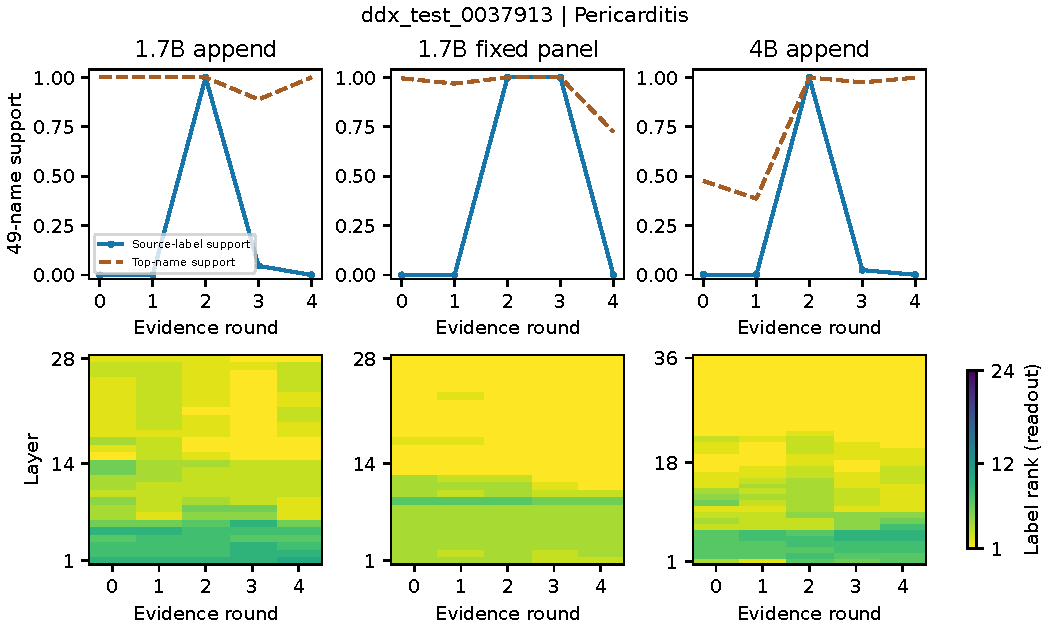
\includegraphics[width=.96\linewidth]{figures/ddx_test_0037913.pdf}\end{center}

{\small\begin{longtable}{>{\raggedright\arraybackslash}p{.07\textwidth}>{\raggedright\arraybackslash}p{.415\textwidth}>{\raggedright\arraybackslash}p{.415\textwidth}}\toprule Round & Newly revealed source evidence & Native top / label support / final-layer probe top \\ \midrule\endhead

0 & Do you have pain somewhere, related to your reason for consulting? Yes; Characterize your pain: a knife stroke; sharp; Do you feel pain somewhere? lower chest; breast(R); How intense is the pain? Recorded scale value 6 on the dataset's 0-10 scale; endpoint meanings are unspecified; Does the pain radiate to another location? thoracic spine; posterior chest wall(R); How precisely is the pain located? Recorded scale value 8 on the dataset's 0-10 scale; endpoint meanings are unspecified; How fast did the pain appear? Recorded scale value 6 on the dataset's 0-10 scale; endpoint meanings are unspecified & 1.7B append: Boerhaave / 0.0000 / Pulmonary embolism\newline 1.7B panel: Acute COPD exacerbation / infection / 0.0000 / Pericarditis\newline 4B append: Bronchospasm / acute asthma exacerbation / 0.0020 / Pericarditis \\ 

1 & Do you have pain that is increased when you breathe in deeply? Yes & 1.7B append: Boerhaave / 0.0000 / Pulmonary embolism\newline 1.7B panel: Acute COPD exacerbation / infection / 0.0000 / Pericarditis\newline 4B append: Pneumonia / 0.0025 / Pericarditis \\ 

2 & Have you ever had a pericarditis? Yes & 1.7B append: Pericarditis / 1.0000 / SLE\newline 1.7B panel: Pericarditis / 1.0000 / Pericarditis\newline 4B append: Pericarditis / 0.9994 / Pericarditis \\ 

3 & Have you recently had a viral infection? Yes & 1.7B append: Acute laryngitis / 0.0467 / Pericarditis\newline 1.7B panel: Pericarditis / 1.0000 / Pericarditis\newline 4B append: Myocarditis / 0.0252 / Pericarditis \\ 

4 & Have you traveled out of the country in the last 4 weeks? No & 1.7B append: Boerhaave / 0.0000 / Pericarditis\newline 1.7B panel: Acute COPD exacerbation / infection / 0.0013 / Pericarditis\newline 4B append: Myocarditis / 0.0014 / Pericarditis \\ 

\bottomrule\end{longtable}}

\clearpage\subsection{ddx\_test\_0041136 -- Acute otitis media}
\label{case:ddx_test_0041136}

Source label: Acute otitis media. Family: ent. Evidence updates: 5. All facts below are source-recorded; their order is acquisition order.

\begin{center}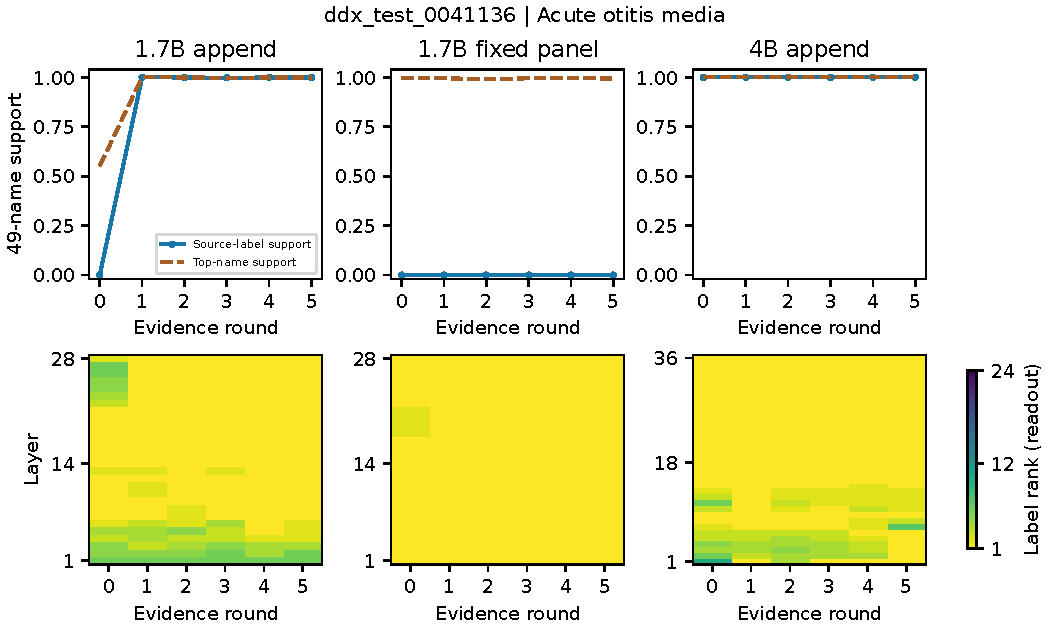
\includegraphics[width=.96\linewidth]{figures/ddx_test_0041136.pdf}\end{center}

{\small\begin{longtable}{>{\raggedright\arraybackslash}p{.07\textwidth}>{\raggedright\arraybackslash}p{.415\textwidth}>{\raggedright\arraybackslash}p{.415\textwidth}}\toprule Round & Newly revealed source evidence & Native top / label support / final-layer probe top \\ \midrule\endhead

0 & Do you have pain somewhere, related to your reason for consulting? Yes; Characterize your pain: sensitive; sharp; Do you feel pain somewhere? ear(R); How intense is the pain? Recorded scale value 6 on the dataset's 0-10 scale; endpoint meanings are unspecified; Does the pain radiate to another location? nowhere; How precisely is the pain located? Recorded scale value 9 on the dataset's 0-10 scale; endpoint meanings are unspecified; How fast did the pain appear? Recorded scale value 3 on the dataset's 0-10 scale; endpoint meanings are unspecified & 1.7B append: Acute laryngitis / 0.0000 / Cluster headache\newline 1.7B panel: Acute COPD exacerbation / infection / 0.0000 / Acute otitis media\newline 4B append: Acute otitis media / 1.0000 / Acute otitis media \\ 

1 & Are you currently being treated or have you recently been treated with an oral antibiotic for an ear infection? Yes & 1.7B append: Acute otitis media / 1.0000 / Acute otitis media\newline 1.7B panel: Acute COPD exacerbation / infection / 0.0001 / Acute otitis media\newline 4B append: Acute otitis media / 1.0000 / Acute otitis media \\ 

2 & Do you have a fever (either felt or measured with a thermometer)? Yes & 1.7B append: Acute otitis media / 0.9998 / Acute otitis media\newline 1.7B panel: Acute COPD exacerbation / infection / 0.0001 / Acute otitis media\newline 4B append: Acute otitis media / 1.0000 / Acute otitis media \\ 

3 & Do you have a cough? Yes & 1.7B append: Acute otitis media / 0.9986 / Acute otitis media\newline 1.7B panel: Acute COPD exacerbation / infection / 0.0000 / Acute otitis media\newline 4B append: Acute otitis media / 1.0000 / Acute otitis media \\ 

4 & Are your vaccinations up to date? Yes & 1.7B append: Acute otitis media / 0.9995 / Acute otitis media\newline 1.7B panel: Acute COPD exacerbation / infection / 0.0000 / Acute otitis media\newline 4B append: Acute otitis media / 1.0000 / Acute otitis media \\ 

5 & Have you traveled out of the country in the last 4 weeks? No & 1.7B append: Acute otitis media / 0.9996 / Acute otitis media\newline 1.7B panel: Acute COPD exacerbation / infection / 0.0000 / Acute otitis media\newline 4B append: Acute otitis media / 1.0000 / Acute otitis media \\ 

\bottomrule\end{longtable}}

\clearpage\subsection{ddx\_test\_0042118 -- Bronchitis}
\label{case:ddx_test_0042118}

Source label: Bronchitis. Family: respiratory. Evidence updates: 8. All facts below are source-recorded; their order is acquisition order.

\begin{center}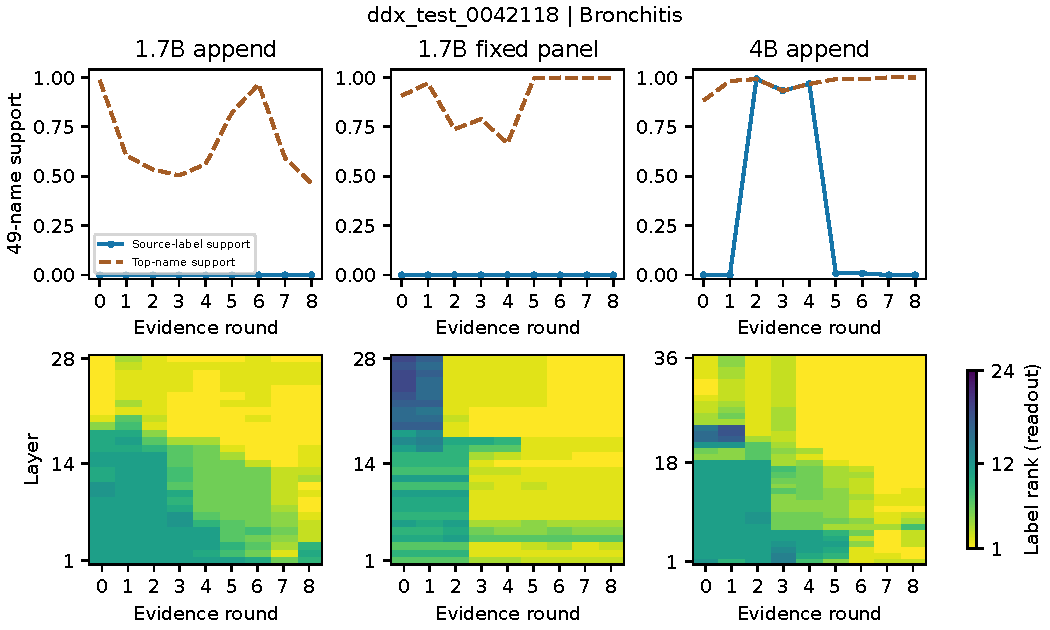
\includegraphics[width=.96\linewidth]{figures/ddx_test_0042118.pdf}\end{center}

{\small\begin{longtable}{>{\raggedright\arraybackslash}p{.07\textwidth}>{\raggedright\arraybackslash}p{.415\textwidth}>{\raggedright\arraybackslash}p{.415\textwidth}}\toprule Round & Newly revealed source evidence & Native top / label support / final-layer probe top \\ \midrule\endhead

0 & Are your symptoms more prominent at night? Yes & 1.7B append: Acute COPD exacerbation / infection / 0.0000 / Bronchitis\newline 1.7B panel: Acute COPD exacerbation / infection / 0.0000 / Guillain-Barr\'{e} syndrome\newline 4B append: Acute rhinosinusitis / 0.0006 / URTI \\ 

1 & Have you traveled out of the country in the last 4 weeks? No & 1.7B append: Acute rhinosinusitis / 0.0000 / Acute otitis media\newline 1.7B panel: Acute COPD exacerbation / infection / 0.0000 / Guillain-Barr\'{e} syndrome\newline 4B append: Acute rhinosinusitis / 0.0001 / URTI \\ 

2 & Have you noticed a wheezing sound when you exhale? Yes & 1.7B append: Bronchiolitis / 0.0000 / Bronchospasm / acute asthma exacerbation\newline 1.7B panel: Whooping cough / 0.0000 / Bronchospasm / acute asthma exacerbation\newline 4B append: Bronchitis / 0.9918 / Bronchospasm / acute asthma exacerbation \\ 

3 & Do you have pain somewhere, related to your reason for consulting? Yes; Characterize your pain: sensitive; Do you feel pain somewhere? lower chest; side of the chest(R); upper chest; breast(L); posterior chest wall(R); How intense is the pain? Recorded scale value 5 on the dataset's 0-10 scale; endpoint meanings are unspecified; Does the pain radiate to another location? nowhere; How precisely is the pain located? Recorded scale value 4 on the dataset's 0-10 scale; endpoint meanings are unspecified; How fast did the pain appear? Recorded scale value 1 on the dataset's 0-10 scale; endpoint meanings are unspecified & 1.7B append: Bronchospasm / acute asthma exacerbation / 0.0000 / Bronchitis\newline 1.7B panel: Acute COPD exacerbation / infection / 0.0000 / Bronchospasm / acute asthma exacerbation\newline 4B append: Bronchitis / 0.9327 / Bronchospasm / acute asthma exacerbation \\ 

4 & Do you have a cough that produces colored or more abundant sputum than usual? Yes & 1.7B append: Bronchospasm / acute asthma exacerbation / 0.0000 / Bronchitis\newline 1.7B panel: Acute COPD exacerbation / infection / 0.0000 / Bronchospasm / acute asthma exacerbation\newline 4B append: Bronchitis / 0.9668 / Bronchitis \\ 

5 & Do you have a chronic obstructive pulmonary disease (COPD)? Yes & 1.7B append: Bronchospasm / acute asthma exacerbation / 0.0000 / Bronchitis\newline 1.7B panel: Acute COPD exacerbation / infection / 0.0000 / Bronchospasm / acute asthma exacerbation\newline 4B append: Acute COPD exacerbation / infection / 0.0086 / Bronchitis \\ 

6 & Do you have a cough? Yes & 1.7B append: Bronchospasm / acute asthma exacerbation / 0.0000 / Bronchospasm / acute asthma exacerbation\newline 1.7B panel: Acute COPD exacerbation / infection / 0.0000 / Bronchitis\newline 4B append: Acute COPD exacerbation / infection / 0.0091 / Bronchitis \\ 

7 & Are you experiencing shortness of breath or difficulty breathing in a significant way? Yes & 1.7B append: Acute COPD exacerbation / infection / 0.0000 / Bronchitis\newline 1.7B panel: Acute COPD exacerbation / infection / 0.0000 / Bronchitis\newline 4B append: Acute COPD exacerbation / infection / 0.0000 / Bronchitis \\ 

8 & Are your vaccinations up to date? Yes & 1.7B append: Acute COPD exacerbation / infection / 0.0000 / Bronchitis\newline 1.7B panel: Acute COPD exacerbation / infection / 0.0000 / Bronchitis\newline 4B append: Acute COPD exacerbation / infection / 0.0002 / Bronchitis \\ 

\bottomrule\end{longtable}}

\clearpage\subsection{ddx\_test\_0044249 -- Boerhaave}
\label{case:ddx_test_0044249}

Source label: Boerhaave. Family: digestive. Evidence updates: 5. All facts below are source-recorded; their order is acquisition order.

\begin{center}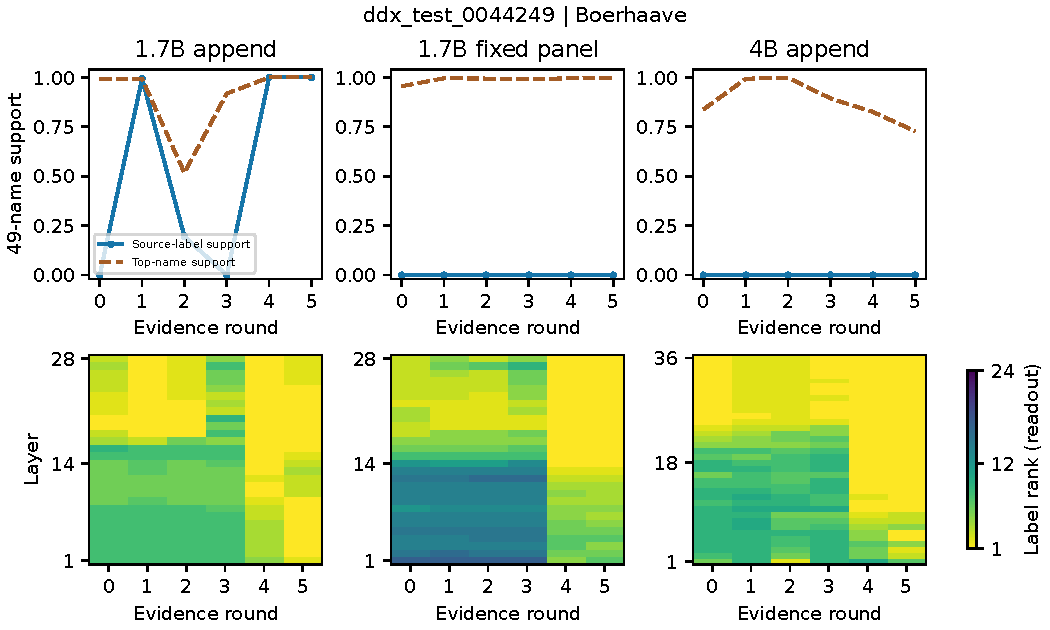
\includegraphics[width=.96\linewidth]{figures/ddx_test_0044249.pdf}\end{center}

{\small\begin{longtable}{>{\raggedright\arraybackslash}p{.07\textwidth}>{\raggedright\arraybackslash}p{.415\textwidth}>{\raggedright\arraybackslash}p{.415\textwidth}}\toprule Round & Newly revealed source evidence & Native top / label support / final-layer probe top \\ \midrule\endhead

0 & Have you vomited several times or have you made several efforts to vomit? Yes & 1.7B append: Acute COPD exacerbation / infection / 0.0000 / GERD\newline 1.7B panel: Acute COPD exacerbation / infection / 0.0000 / Bronchospasm / acute asthma exacerbation\newline 4B append: Acute rhinosinusitis / 0.0000 / Boerhaave \\ 

1 & Are you feeling nauseous or do you feel like vomiting? Yes & 1.7B append: Boerhaave / 0.9932 / Boerhaave\newline 1.7B panel: Acute COPD exacerbation / infection / 0.0000 / Acute dystonic reactions\newline 4B append: Acute rhinosinusitis / 0.0000 / URTI \\ 

2 & Have you traveled out of the country in the last 4 weeks? No & 1.7B append: Acute COPD exacerbation / infection / 0.1947 / GERD\newline 1.7B panel: Acute COPD exacerbation / infection / 0.0000 / Acute dystonic reactions\newline 4B append: Acute rhinosinusitis / 0.0000 / URTI \\ 

3 & Do you drink alcohol excessively or do you have an addiction to alcohol? Yes & 1.7B append: GERD / 0.0000 / GERD\newline 1.7B panel: Acute COPD exacerbation / infection / 0.0000 / Acute dystonic reactions\newline 4B append: Acute rhinosinusitis / 0.0000 / Boerhaave \\ 

4 & Do you have pain somewhere, related to your reason for consulting? Yes; Characterize your pain: heartbreaking; haunting; a knife stroke; violent; sickening; Do you feel pain somewhere? lower chest; flank(R); flank(L); upper chest; epigastric; How intense is the pain? Recorded scale value 6 on the dataset's 0-10 scale; endpoint meanings are unspecified; Does the pain radiate to another location? thoracic spine; scapula(R); scapula(L); How precisely is the pain located? Recorded scale value 2 on the dataset's 0-10 scale; endpoint meanings are unspecified; How fast did the pain appear? Recorded scale value 7 on the dataset's 0-10 scale; endpoint meanings are unspecified & 1.7B append: Boerhaave / 1.0000 / Boerhaave\newline 1.7B panel: Acute COPD exacerbation / infection / 0.0000 / Boerhaave\newline 4B append: Pneumonia / 0.0000 / Boerhaave \\ 

5 & Have you recently thrown up blood or something resembling coffee beans? Yes & 1.7B append: Boerhaave / 0.9999 / GERD\newline 1.7B panel: Acute COPD exacerbation / infection / 0.0000 / Boerhaave\newline 4B append: Pulmonary embolism / 0.0000 / Boerhaave \\ 

\bottomrule\end{longtable}}

\clearpage\subsection{ddx\_test\_0045887 -- URTI}
\label{case:ddx_test_0045887}

Source label: URTI. Family: ent. Evidence updates: 10. All facts below are source-recorded; their order is acquisition order.

\begin{center}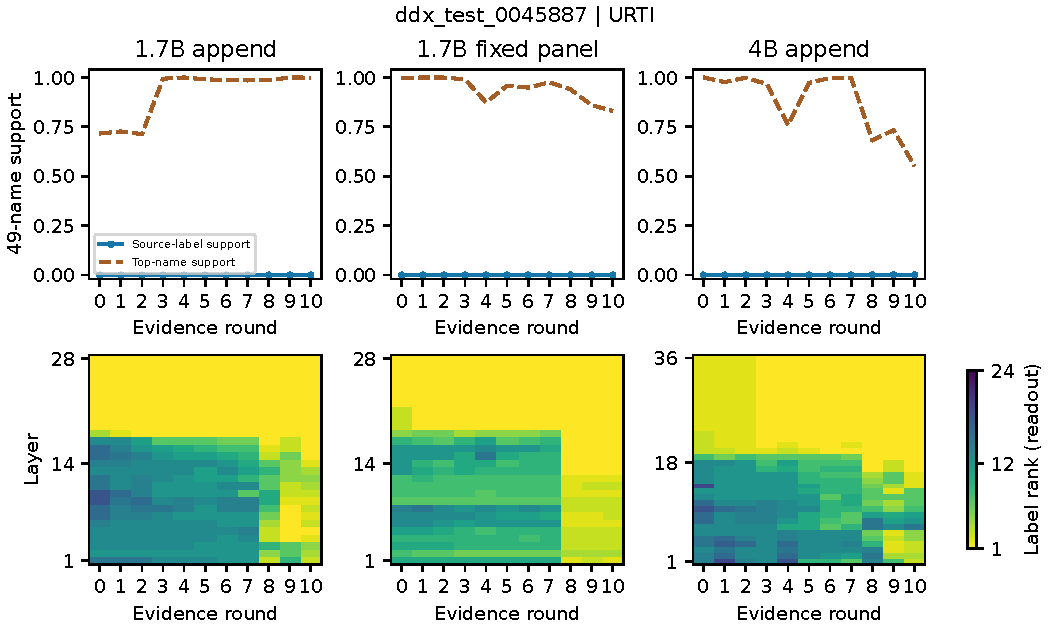
\includegraphics[width=.96\linewidth]{figures/ddx_test_0045887.pdf}\end{center}

{\small\begin{longtable}{>{\raggedright\arraybackslash}p{.07\textwidth}>{\raggedright\arraybackslash}p{.415\textwidth}>{\raggedright\arraybackslash}p{.415\textwidth}}\toprule Round & Newly revealed source evidence & Native top / label support / final-layer probe top \\ \midrule\endhead

0 & Do you have a sore throat? Yes & 1.7B append: Acute rhinosinusitis / 0.0000 / URTI\newline 1.7B panel: Acute COPD exacerbation / infection / 0.0000 / URTI\newline 4B append: Viral pharyngitis / 0.0000 / Viral pharyngitis \\ 

1 & Are you exposed to secondhand cigarette smoke on a daily basis? Yes & 1.7B append: Acute laryngitis / 0.0000 / URTI\newline 1.7B panel: Acute COPD exacerbation / infection / 0.0000 / URTI\newline 4B append: Viral pharyngitis / 0.0000 / Viral pharyngitis \\ 

2 & Do you have diffuse (widespread) muscle pain? Yes & 1.7B append: Acute rhinosinusitis / 0.0000 / URTI\newline 1.7B panel: Acute COPD exacerbation / infection / 0.0000 / URTI\newline 4B append: Viral pharyngitis / 0.0000 / Viral pharyngitis \\ 

3 & Do you have nasal congestion or a clear runny nose? Yes & 1.7B append: Acute rhinosinusitis / 0.0000 / URTI\newline 1.7B panel: Acute COPD exacerbation / infection / 0.0000 / URTI\newline 4B append: Viral pharyngitis / 0.0000 / URTI \\ 

4 & Do you have a cough that produces colored or more abundant sputum than usual? Yes & 1.7B append: Acute rhinosinusitis / 0.0000 / URTI\newline 1.7B panel: Acute COPD exacerbation / infection / 0.0000 / URTI\newline 4B append: Influenza / 0.0002 / URTI \\ 

5 & Have you had significantly increased sweating? Yes & 1.7B append: Acute rhinosinusitis / 0.0000 / URTI\newline 1.7B panel: Acute COPD exacerbation / infection / 0.0000 / URTI\newline 4B append: Influenza / 0.0000 / URTI \\ 

6 & Have you traveled out of the country in the last 4 weeks? No & 1.7B append: Acute rhinosinusitis / 0.0000 / URTI\newline 1.7B panel: Acute COPD exacerbation / infection / 0.0000 / URTI\newline 4B append: Influenza / 0.0000 / URTI \\ 

7 & Do you have a cough? Yes & 1.7B append: Acute rhinosinusitis / 0.0000 / URTI\newline 1.7B panel: Acute COPD exacerbation / infection / 0.0000 / URTI\newline 4B append: Influenza / 0.0000 / URTI \\ 

8 & Do you have pain somewhere, related to your reason for consulting? Yes; Characterize your pain: tedious; Do you feel pain somewhere? forehead; cheek(R); cheek(L); temple(R); How intense is the pain? Recorded scale value 2 on the dataset's 0-10 scale; endpoint meanings are unspecified; Does the pain radiate to another location? nowhere; How precisely is the pain located? Recorded scale value 5 on the dataset's 0-10 scale; endpoint meanings are unspecified; How fast did the pain appear? Recorded scale value 2 on the dataset's 0-10 scale; endpoint meanings are unspecified & 1.7B append: Acute rhinosinusitis / 0.0000 / URTI\newline 1.7B panel: Acute COPD exacerbation / infection / 0.0000 / URTI\newline 4B append: Influenza / 0.0006 / URTI \\ 

9 & Have you been in contact with a person with similar symptoms in the past 2 weeks? Yes & 1.7B append: Acute rhinosinusitis / 0.0000 / URTI\newline 1.7B panel: Acute COPD exacerbation / infection / 0.0000 / URTI\newline 4B append: Viral pharyngitis / 0.0014 / URTI \\ 

10 & Do you live with 4 or more people? Yes & 1.7B append: Acute rhinosinusitis / 0.0000 / URTI\newline 1.7B panel: Acute COPD exacerbation / infection / 0.0000 / URTI\newline 4B append: Viral pharyngitis / 0.0005 / URTI \\ 

\bottomrule\end{longtable}}

\clearpage\subsection{ddx\_test\_0048692 -- Pulmonary embolism}
\label{case:ddx_test_0048692}

Source label: Pulmonary embolism. Family: respiratory. Evidence updates: 6. All facts below are source-recorded; their order is acquisition order.

\begin{center}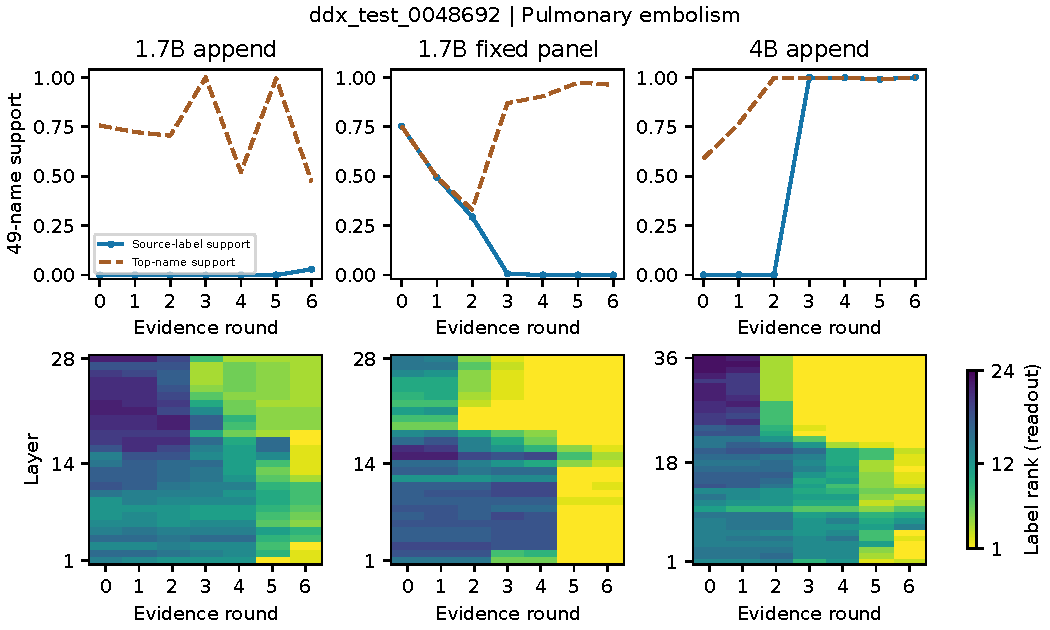
\includegraphics[width=.96\linewidth]{figures/ddx_test_0048692.pdf}\end{center}

{\small\begin{longtable}{>{\raggedright\arraybackslash}p{.07\textwidth}>{\raggedright\arraybackslash}p{.415\textwidth}>{\raggedright\arraybackslash}p{.415\textwidth}}\toprule Round & Newly revealed source evidence & Native top / label support / final-layer probe top \\ \midrule\endhead

0 & Do you have pain that is increased when you breathe in deeply? Yes & 1.7B append: Acute COPD exacerbation / infection / 0.0000 / Bronchitis\newline 1.7B panel: Pulmonary embolism / 0.7534 / SLE\newline 4B append: Acute pulmonary edema / 0.0000 / Bronchitis \\ 

1 & Have you traveled out of the country in the last 4 weeks? No & 1.7B append: Acute rhinosinusitis / 0.0016 / Bronchitis\newline 1.7B panel: Pulmonary embolism / 0.4941 / SLE\newline 4B append: Bronchitis / 0.0025 / Bronchitis \\ 

2 & Have you been coughing up blood? Yes & 1.7B append: Bronchiolitis / 0.0001 / Bronchitis\newline 1.7B panel: Acute COPD exacerbation / infection / 0.2943 / SLE\newline 4B append: Pneumonia / 0.0020 / Pneumonia \\ 

3 & Do you have swelling in one or more areas of your body? Yes; Where is the swelling located? posterior aspect of the ankle(R); posterior aspect of the ankle(L) & 1.7B append: Localized edema / 0.0000 / Acute pulmonary edema\newline 1.7B panel: Acute COPD exacerbation / infection / 0.0067 / SLE\newline 4B append: Pulmonary embolism / 0.9991 / Pulmonary embolism \\ 

4 & Did you lose consciousness? Yes & 1.7B append: Acute pulmonary edema / 0.0009 / Acute pulmonary edema\newline 1.7B panel: Acute COPD exacerbation / infection / 0.0002 / Pulmonary embolism\newline 4B append: Pulmonary embolism / 0.9984 / Pulmonary embolism \\ 

5 & Do you have pain somewhere, related to your reason for consulting? Yes; Characterize your pain: sharp; Do you feel pain somewhere? side of the chest(R); side of the chest(L); scapula(R); scapula(L); posterior chest wall(R); How intense is the pain? Recorded scale value 1 on the dataset's 0-10 scale; endpoint meanings are unspecified; Does the pain radiate to another location? side of the chest(L); upper chest; scapula(R); breast(R); posterior chest wall(L); How precisely is the pain located? Recorded scale value 9 on the dataset's 0-10 scale; endpoint meanings are unspecified; How fast did the pain appear? Recorded scale value 3 on the dataset's 0-10 scale; endpoint meanings are unspecified & 1.7B append: Localized edema / 0.0001 / Acute pulmonary edema\newline 1.7B panel: Acute COPD exacerbation / infection / 0.0000 / Pulmonary embolism\newline 4B append: Pulmonary embolism / 0.9906 / Pulmonary embolism \\ 

6 & Have you ever had deep vein thrombosis (DVT)? Yes & 1.7B append: Acute pulmonary edema / 0.0297 / Spontaneous pneumothorax\newline 1.7B panel: Acute COPD exacerbation / infection / 0.0000 / Pulmonary embolism\newline 4B append: Pulmonary embolism / 1.0000 / Pulmonary embolism \\ 

\bottomrule\end{longtable}}

\clearpage\subsection{ddx\_test\_0060159 -- Acute dystonic reactions}
\label{case:ddx_test_0060159}

Source label: Acute dystonic reactions. Family: neurologic. Evidence updates: 8. All facts below are source-recorded; their order is acquisition order.

\begin{center}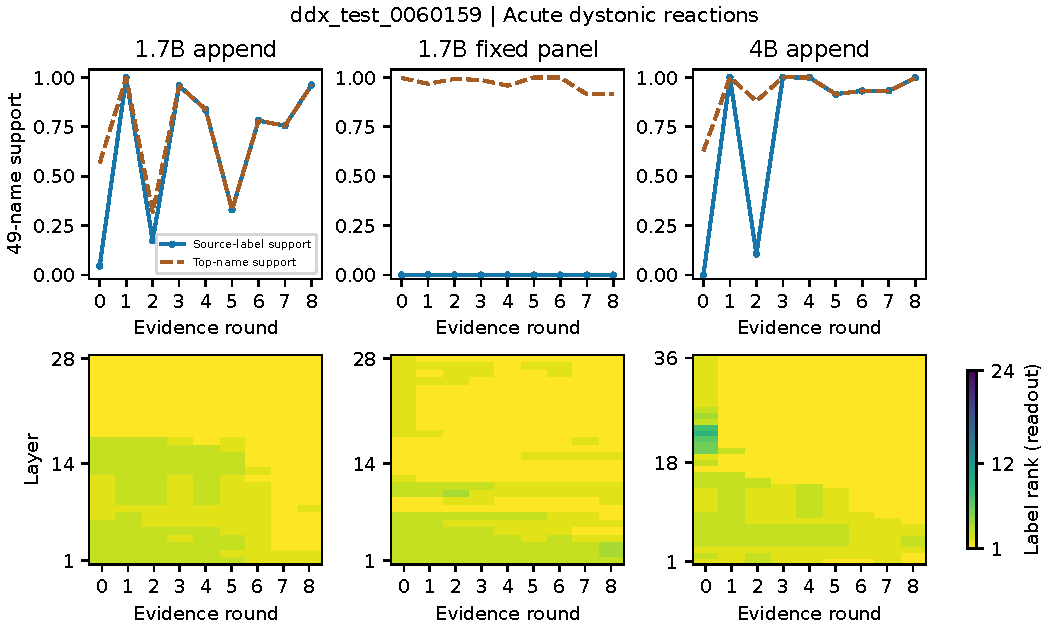
\includegraphics[width=.96\linewidth]{figures/ddx_test_0060159.pdf}\end{center}

{\small\begin{longtable}{>{\raggedright\arraybackslash}p{.07\textwidth}>{\raggedright\arraybackslash}p{.415\textwidth}>{\raggedright\arraybackslash}p{.415\textwidth}}\toprule Round & Newly revealed source evidence & Native top / label support / final-layer probe top \\ \midrule\endhead

0 & Do you feel that muscle spasms or soreness in your neck are keeping you from turning your head to one side? Yes & 1.7B append: Acute laryngitis / 0.0458 / Acute dystonic reactions\newline 1.7B panel: Acute COPD exacerbation / infection / 0.0001 / Myasthenia gravis\newline 4B append: Acute otitis media / 0.0000 / URTI \\ 

1 & Have you started or taken any antipsychotic medication within the last 7 days? Yes & 1.7B append: Acute dystonic reactions / 0.9990 / Acute dystonic reactions\newline 1.7B panel: Acute COPD exacerbation / infection / 0.0028 / Acute dystonic reactions\newline 4B append: Acute dystonic reactions / 1.0000 / Acute dystonic reactions \\ 

2 & Are you experiencing shortness of breath or difficulty breathing in a significant way? Yes & 1.7B append: Acute COPD exacerbation / infection / 0.1732 / Acute dystonic reactions\newline 1.7B panel: Acute pulmonary edema / 0.0000 / Acute dystonic reactions\newline 4B append: Acute pulmonary edema / 0.1068 / Acute dystonic reactions \\ 

3 & Do you have annoying muscle spasms in your face, neck or any other part of your body? Yes & 1.7B append: Acute dystonic reactions / 0.9577 / Acute dystonic reactions\newline 1.7B panel: Acute pulmonary edema / 0.0000 / Acute dystonic reactions\newline 4B append: Acute dystonic reactions / 0.9999 / Acute dystonic reactions \\ 

4 & Do you suddenly have difficulty or an inability to open your mouth or have jaw pain when opening it? Yes & 1.7B append: Acute dystonic reactions / 0.8381 / Acute dystonic reactions\newline 1.7B panel: Acute pulmonary edema / 0.0000 / Acute dystonic reactions\newline 4B append: Acute dystonic reactions / 0.9997 / Acute dystonic reactions \\ 

5 & Have you ever felt like you were suffocating for a very short time associated with inability to breathe or speak? Yes & 1.7B append: Acute dystonic reactions / 0.3305 / Acute dystonic reactions\newline 1.7B panel: Acute pulmonary edema / 0.0000 / Acute dystonic reactions\newline 4B append: Acute dystonic reactions / 0.9153 / Acute dystonic reactions \\ 

6 & Have you been treated in hospital recently for nausea, agitation, intoxication or aggressive behavior and received medication via an intravenous or intramuscular route? Yes & 1.7B append: Acute dystonic reactions / 0.7815 / Acute dystonic reactions\newline 1.7B panel: Acute pulmonary edema / 0.0000 / Acute dystonic reactions\newline 4B append: Acute dystonic reactions / 0.9318 / Acute dystonic reactions \\ 

7 & Do you regularly take stimulant drugs? Yes & 1.7B append: Acute dystonic reactions / 0.7554 / Acute dystonic reactions\newline 1.7B panel: Acute pulmonary edema / 0.0000 / Acute dystonic reactions\newline 4B append: Acute dystonic reactions / 0.9320 / Acute dystonic reactions \\ 

8 & Have you traveled out of the country in the last 4 weeks? No & 1.7B append: Acute dystonic reactions / 0.9620 / Acute dystonic reactions\newline 1.7B panel: Acute pulmonary edema / 0.0001 / Acute dystonic reactions\newline 4B append: Acute dystonic reactions / 0.9979 / Acute dystonic reactions \\ 

\bottomrule\end{longtable}}

\clearpage\subsection{ddx\_test\_0061730 -- Cluster headache}
\label{case:ddx_test_0061730}

Source label: Cluster headache. Family: neurologic. Evidence updates: 4. All facts below are source-recorded; their order is acquisition order.

\begin{center}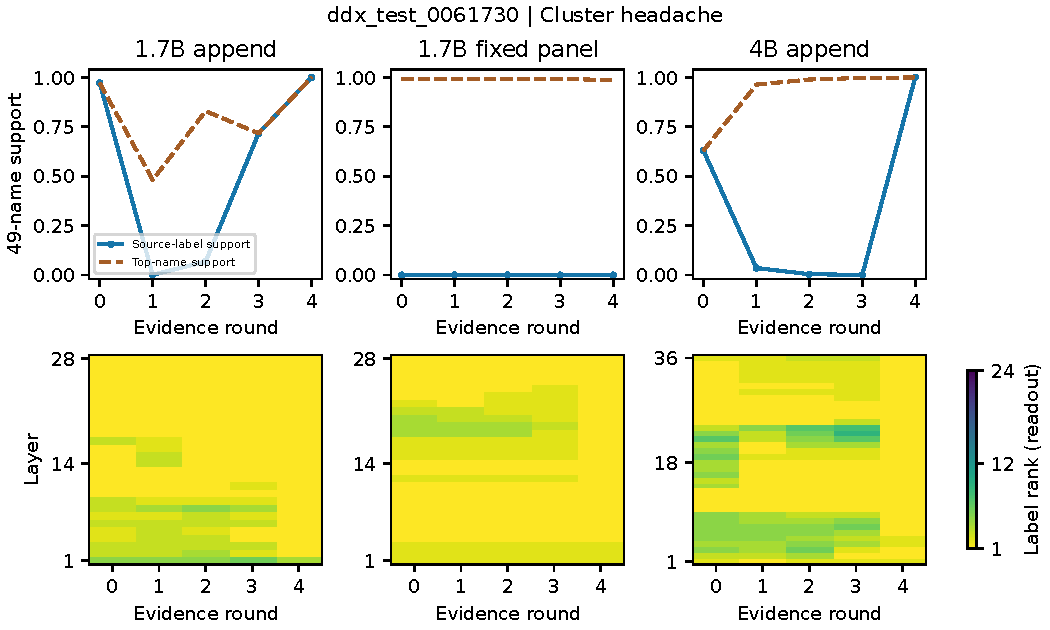
\includegraphics[width=.96\linewidth]{figures/ddx_test_0061730.pdf}\end{center}

{\small\begin{longtable}{>{\raggedright\arraybackslash}p{.07\textwidth}>{\raggedright\arraybackslash}p{.415\textwidth}>{\raggedright\arraybackslash}p{.415\textwidth}}\toprule Round & Newly revealed source evidence & Native top / label support / final-layer probe top \\ \midrule\endhead

0 & Do you have pain somewhere, related to your reason for consulting? Yes; Characterize your pain: haunting; a knife stroke; tugging; violent; sharp; Do you feel pain somewhere? forehead; cheek(R); cheek(L); eye(R); eye(L); How intense is the pain? Recorded scale value 9 on the dataset's 0-10 scale; endpoint meanings are unspecified; Does the pain radiate to another location? nowhere; How precisely is the pain located? Recorded scale value 10 on the dataset's 0-10 scale; endpoint meanings are unspecified; How fast did the pain appear? Recorded scale value 9 on the dataset's 0-10 scale; endpoint meanings are unspecified & 1.7B append: Cluster headache / 0.9719 / Cluster headache\newline 1.7B panel: Acute COPD exacerbation / infection / 0.0000 / Cluster headache\newline 4B append: Cluster headache / 0.6298 / SLE \\ 

1 & Do you drink alcohol excessively or do you have an addiction to alcohol? Yes & 1.7B append: Acute rhinosinusitis / 0.0010 / Cluster headache\newline 1.7B panel: Acute COPD exacerbation / infection / 0.0000 / Cluster headache\newline 4B append: Acute rhinosinusitis / 0.0357 / SLE \\ 

2 & Have you traveled out of the country in the last 4 weeks? No & 1.7B append: Acute rhinosinusitis / 0.0683 / Cluster headache\newline 1.7B panel: Acute COPD exacerbation / infection / 0.0000 / Cluster headache\newline 4B append: Acute rhinosinusitis / 0.0043 / SLE \\ 

3 & Do you take medication that dilates your blood vessels? Yes & 1.7B append: Cluster headache / 0.7170 / Cluster headache\newline 1.7B panel: Acute COPD exacerbation / infection / 0.0000 / Cluster headache\newline 4B append: Acute rhinosinusitis / 0.0010 / SLE \\ 

4 & Have any of your family members been diagnosed with cluster headaches? Yes & 1.7B append: Cluster headache / 1.0000 / Cluster headache\newline 1.7B panel: Acute COPD exacerbation / infection / 0.0000 / Cluster headache\newline 4B append: Cluster headache / 1.0000 / Cluster headache \\ 

\bottomrule\end{longtable}}

\clearpage\subsection{ddx\_test\_0062355 -- Acute dystonic reactions}
\label{case:ddx_test_0062355}

Source label: Acute dystonic reactions. Family: neurologic. Evidence updates: 8. All facts below are source-recorded; their order is acquisition order.

\begin{center}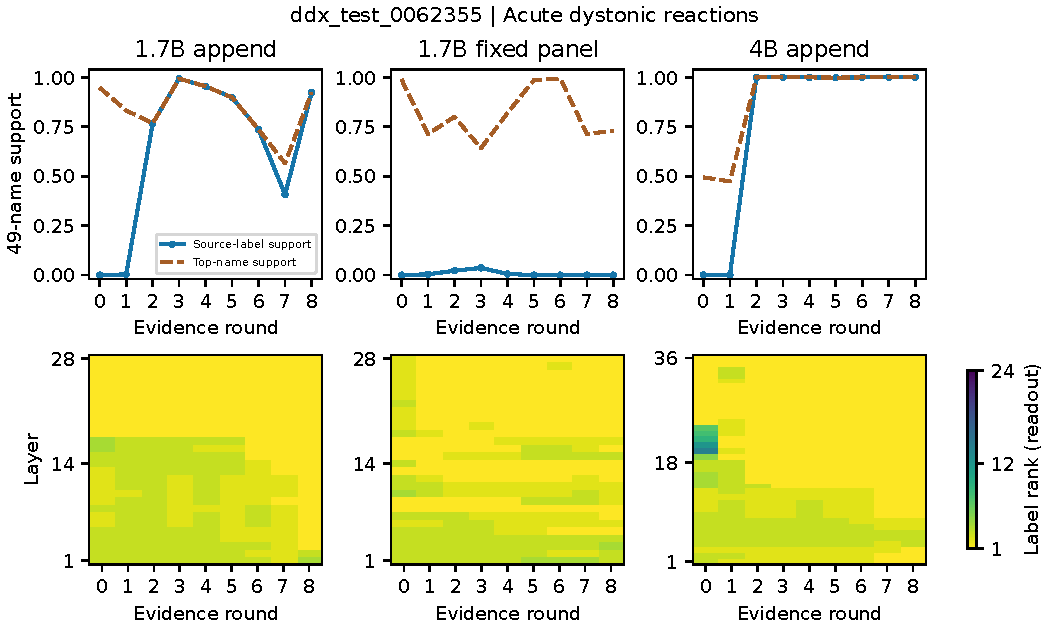
\includegraphics[width=.96\linewidth]{figures/ddx_test_0062355.pdf}\end{center}

{\small\begin{longtable}{>{\raggedright\arraybackslash}p{.07\textwidth}>{\raggedright\arraybackslash}p{.415\textwidth}>{\raggedright\arraybackslash}p{.415\textwidth}}\toprule Round & Newly revealed source evidence & Native top / label support / final-layer probe top \\ \midrule\endhead

0 & Are you unable to control the direction of your eyes? Yes & 1.7B append: Acute COPD exacerbation / infection / 0.0001 / Acute dystonic reactions\newline 1.7B panel: Acute COPD exacerbation / infection / 0.0000 / Myasthenia gravis\newline 4B append: Acute rhinosinusitis / 0.0012 / Acute dystonic reactions \\ 

1 & Do you suddenly have difficulty or an inability to open your mouth or have jaw pain when opening it? Yes & 1.7B append: Acute laryngitis / 0.0034 / Acute dystonic reactions\newline 1.7B panel: Acute COPD exacerbation / infection / 0.0037 / Acute dystonic reactions\newline 4B append: Acute rhinosinusitis / 0.0000 / Acute dystonic reactions \\ 

2 & Have you started or taken any antipsychotic medication within the last 7 days? Yes & 1.7B append: Acute dystonic reactions / 0.7669 / Acute dystonic reactions\newline 1.7B panel: Acute laryngitis / 0.0220 / Acute dystonic reactions\newline 4B append: Acute dystonic reactions / 1.0000 / Acute dystonic reactions \\ 

3 & Have you traveled out of the country in the last 4 weeks? No & 1.7B append: Acute dystonic reactions / 0.9938 / Acute dystonic reactions\newline 1.7B panel: Acute laryngitis / 0.0362 / Acute dystonic reactions\newline 4B append: Acute dystonic reactions / 1.0000 / Acute dystonic reactions \\ 

4 & Have you been treated in hospital recently for nausea, agitation, intoxication or aggressive behavior and received medication via an intravenous or intramuscular route? Yes & 1.7B append: Acute dystonic reactions / 0.9547 / Acute dystonic reactions\newline 1.7B panel: Acute COPD exacerbation / infection / 0.0054 / Acute dystonic reactions\newline 4B append: Acute dystonic reactions / 1.0000 / Acute dystonic reactions \\ 

5 & Are you experiencing shortness of breath or difficulty breathing in a significant way? Yes & 1.7B append: Acute dystonic reactions / 0.8985 / Acute dystonic reactions\newline 1.7B panel: Acute pulmonary edema / 0.0000 / Acute dystonic reactions\newline 4B append: Acute dystonic reactions / 0.9990 / Acute dystonic reactions \\ 

6 & Do you have a hard time opening/raising one or both eyelids? Yes & 1.7B append: Acute dystonic reactions / 0.7363 / Acute dystonic reactions\newline 1.7B panel: Acute pulmonary edema / 0.0000 / Acute dystonic reactions\newline 4B append: Acute dystonic reactions / 1.0000 / Acute dystonic reactions \\ 

7 & Do you regularly take stimulant drugs? Yes & 1.7B append: Acute laryngitis / 0.4070 / Acute dystonic reactions\newline 1.7B panel: Acute pulmonary edema / 0.0002 / Acute dystonic reactions\newline 4B append: Acute dystonic reactions / 1.0000 / Acute dystonic reactions \\ 

8 & Do you feel that muscle spasms or soreness in your neck are keeping you from turning your head to one side? Yes & 1.7B append: Acute dystonic reactions / 0.9228 / Acute dystonic reactions\newline 1.7B panel: Acute pulmonary edema / 0.0001 / Acute dystonic reactions\newline 4B append: Acute dystonic reactions / 1.0000 / Acute dystonic reactions \\ 

\bottomrule\end{longtable}}

\clearpage\subsection{ddx\_test\_0064225 -- Acute pulmonary edema}
\label{case:ddx_test_0064225}

Source label: Acute pulmonary edema. Family: respiratory. Evidence updates: 12. All facts below are source-recorded; their order is acquisition order.

\begin{center}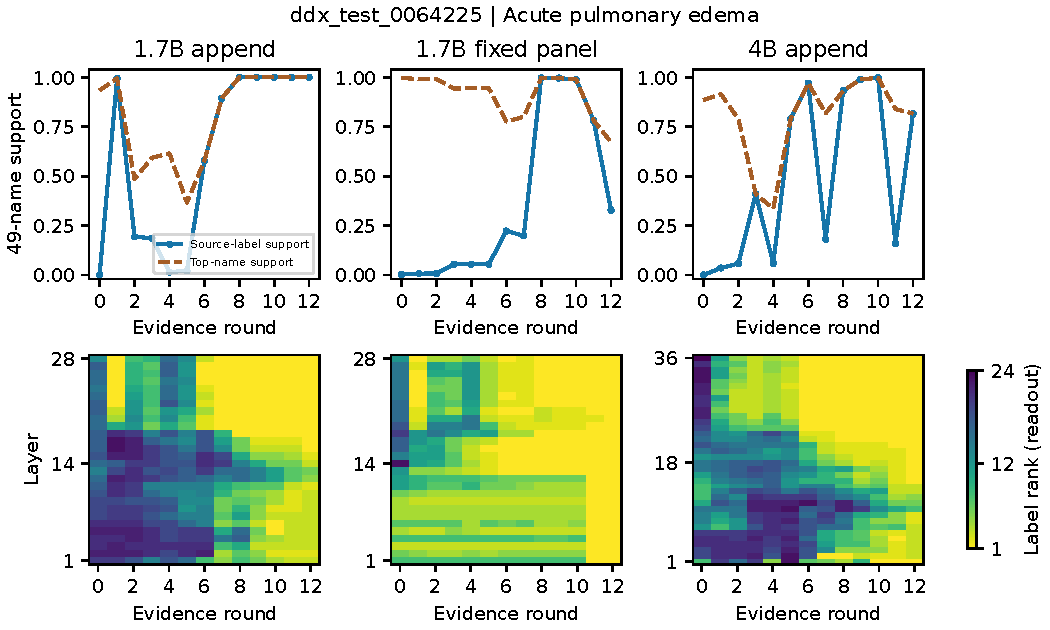
\includegraphics[width=.96\linewidth]{figures/ddx_test_0064225.pdf}\end{center}

{\small\begin{longtable}{>{\raggedright\arraybackslash}p{.07\textwidth}>{\raggedright\arraybackslash}p{.415\textwidth}>{\raggedright\arraybackslash}p{.415\textwidth}}\toprule Round & Newly revealed source evidence & Native top / label support / final-layer probe top \\ \midrule\endhead

0 & Do you have pain somewhere, related to your reason for consulting? Yes; Characterize your pain: sensitive; Do you feel pain somewhere? lower chest; ankle(R); ankle(L); side of the chest(L); breast(R); How intense is the pain? Recorded scale value 2 on the dataset's 0-10 scale; endpoint meanings are unspecified; Does the pain radiate to another location? biceps(R); biceps(L); chin; jaw; shoulder(R); How precisely is the pain located? Recorded scale value 7 on the dataset's 0-10 scale; endpoint meanings are unspecified; How fast did the pain appear? Recorded scale value 1 on the dataset's 0-10 scale; endpoint meanings are unspecified & 1.7B append: Acute rhinosinusitis / 0.0020 / Inguinal hernia\newline 1.7B panel: Acute COPD exacerbation / infection / 0.0027 / Pericarditis\newline 4B append: Acute rhinosinusitis / 0.0001 / Possible NSTEMI / STEMI \\ 

1 & Have you ever had fluid in your lungs? Yes & 1.7B append: Acute pulmonary edema / 0.9951 / Acute pulmonary edema\newline 1.7B panel: Acute COPD exacerbation / infection / 0.0075 / Acute pulmonary edema\newline 4B append: Pneumonia / 0.0356 / Pericarditis \\ 

2 & Do you have symptoms that are increased with physical exertion but alleviated with rest? Yes & 1.7B append: Acute rhinosinusitis / 0.1935 / Bronchitis\newline 1.7B panel: Acute COPD exacerbation / infection / 0.0081 / Stable angina\newline 4B append: Pneumonia / 0.0586 / Pericarditis \\ 

3 & Do you have bouts of choking or shortness of breath that wake you up at night? Yes & 1.7B append: Acute laryngitis / 0.1867 / Bronchitis\newline 1.7B panel: Acute COPD exacerbation / infection / 0.0549 / Stable angina\newline 4B append: Acute pulmonary edema / 0.4096 / Bronchitis \\ 

4 & Have you traveled out of the country in the last 4 weeks? No & 1.7B append: Acute laryngitis / 0.0149 / Bronchitis\newline 1.7B panel: Acute COPD exacerbation / infection / 0.0541 / Stable angina\newline 4B append: Pneumonia / 0.0588 / Bronchitis \\ 

5 & Are your symptoms worse when lying down and alleviated while sitting up? Yes & 1.7B append: Acute laryngitis / 0.0220 / Bronchitis\newline 1.7B panel: Acute COPD exacerbation / infection / 0.0542 / Guillain-Barr\'{e} syndrome\newline 4B append: Acute pulmonary edema / 0.7905 / Bronchitis \\ 

6 & Do you currently undergo dialysis? Yes & 1.7B append: Acute pulmonary edema / 0.5785 / Bronchitis\newline 1.7B panel: Acute COPD exacerbation / infection / 0.2226 / Acute pulmonary edema\newline 4B append: Acute pulmonary edema / 0.9707 / Acute pulmonary edema \\ 

7 & Are you experiencing shortness of breath or difficulty breathing in a significant way? Yes & 1.7B append: Acute pulmonary edema / 0.8950 / Acute pulmonary edema\newline 1.7B panel: Acute COPD exacerbation / infection / 0.1992 / Guillain-Barr\'{e} syndrome\newline 4B append: Pulmonary embolism / 0.1806 / Acute pulmonary edema \\ 

8 & Do you have heart failure? Yes & 1.7B append: Acute pulmonary edema / 1.0000 / Acute pulmonary edema\newline 1.7B panel: Acute pulmonary edema / 0.9974 / Acute pulmonary edema\newline 4B append: Acute pulmonary edema / 0.9318 / Acute pulmonary edema \\ 

9 & Have you had significantly increased sweating? Yes & 1.7B append: Acute pulmonary edema / 1.0000 / Acute pulmonary edema\newline 1.7B panel: Acute pulmonary edema / 0.9966 / Acute pulmonary edema\newline 4B append: Acute pulmonary edema / 0.9906 / Acute pulmonary edema \\ 

10 & Do you have high blood pressure or do you take medications to treat high blood pressure? Yes & 1.7B append: Acute pulmonary edema / 1.0000 / Acute pulmonary edema\newline 1.7B panel: Acute pulmonary edema / 0.9893 / Acute pulmonary edema\newline 4B append: Acute pulmonary edema / 0.9976 / Acute pulmonary edema \\ 

11 & Do you have swelling in one or more areas of your body? Yes; Where is the swelling located? ankle(R); calf(R); calf(L); tibia(L) & 1.7B append: Acute pulmonary edema / 1.0000 / Acute pulmonary edema\newline 1.7B panel: Acute pulmonary edema / 0.7826 / Acute pulmonary edema\newline 4B append: Pulmonary embolism / 0.1604 / Acute pulmonary edema \\ 

12 & Have you ever had a heart attack or do you have angina (chest pain)? Yes & 1.7B append: Acute pulmonary edema / 1.0000 / Acute pulmonary edema\newline 1.7B panel: Acute COPD exacerbation / infection / 0.3277 / Acute pulmonary edema\newline 4B append: Acute pulmonary edema / 0.8167 / Acute pulmonary edema \\ 

\bottomrule\end{longtable}}

\clearpage\subsection{ddx\_test\_0067994 -- Bronchitis}
\label{case:ddx_test_0067994}

Source label: Bronchitis. Family: respiratory. Evidence updates: 9. All facts below are source-recorded; their order is acquisition order.

\begin{center}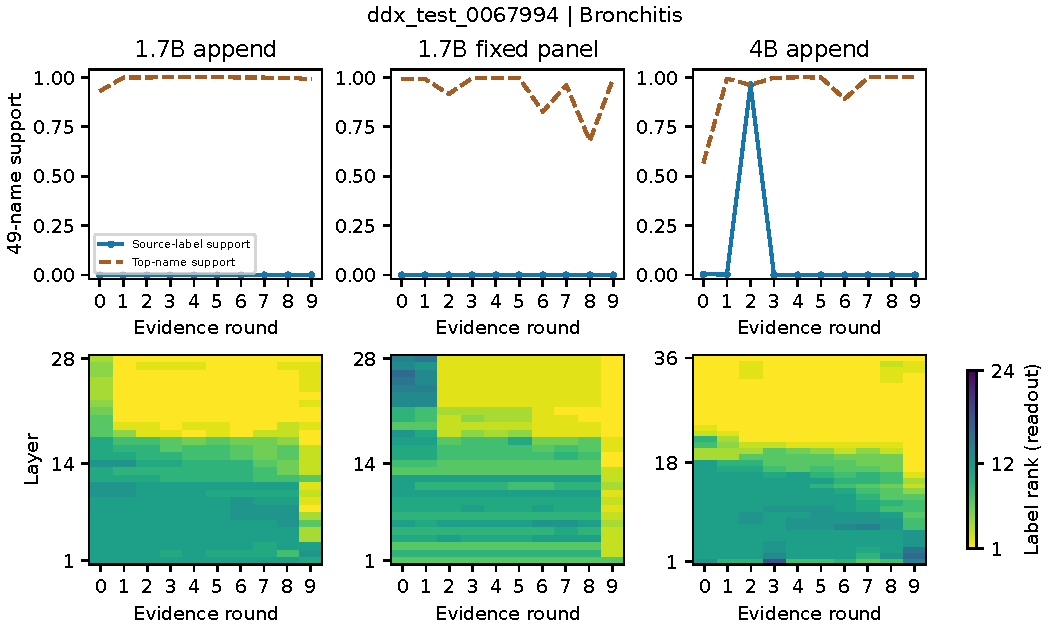
\includegraphics[width=.96\linewidth]{figures/ddx_test_0067994.pdf}\end{center}

{\small\begin{longtable}{>{\raggedright\arraybackslash}p{.07\textwidth}>{\raggedright\arraybackslash}p{.415\textwidth}>{\raggedright\arraybackslash}p{.415\textwidth}}\toprule Round & Newly revealed source evidence & Native top / label support / final-layer probe top \\ \midrule\endhead

0 & Are you experiencing shortness of breath or difficulty breathing in a significant way? Yes & 1.7B append: Acute pulmonary edema / 0.0000 / Acute pulmonary edema\newline 1.7B panel: Acute pulmonary edema / 0.0000 / Guillain-Barr\'{e} syndrome\newline 4B append: Acute COPD exacerbation / infection / 0.0039 / Bronchitis \\ 

1 & Do you smoke cigarettes? Yes & 1.7B append: Acute COPD exacerbation / infection / 0.0000 / Bronchitis\newline 1.7B panel: Acute pulmonary edema / 0.0000 / Guillain-Barr\'{e} syndrome\newline 4B append: Acute COPD exacerbation / infection / 0.0026 / Bronchitis \\ 

2 & Have you noticed a wheezing sound when you exhale? Yes & 1.7B append: Acute COPD exacerbation / infection / 0.0000 / Bronchitis\newline 1.7B panel: Acute pulmonary edema / 0.0000 / Bronchospasm / acute asthma exacerbation\newline 4B append: Bronchitis / 0.9620 / Bronchitis \\ 

3 & Do you have a fever (either felt or measured with a thermometer)? Yes & 1.7B append: Acute COPD exacerbation / infection / 0.0000 / Bronchitis\newline 1.7B panel: Acute pulmonary edema / 0.0000 / Bronchospasm / acute asthma exacerbation\newline 4B append: Acute COPD exacerbation / infection / 0.0000 / Bronchitis \\ 

4 & Are your symptoms more prominent at night? Yes & 1.7B append: Acute COPD exacerbation / infection / 0.0000 / Bronchitis\newline 1.7B panel: Acute pulmonary edema / 0.0000 / Bronchospasm / acute asthma exacerbation\newline 4B append: Acute COPD exacerbation / infection / 0.0000 / Bronchitis \\ 

5 & Have you traveled out of the country in the last 4 weeks? No & 1.7B append: Acute COPD exacerbation / infection / 0.0000 / Bronchitis\newline 1.7B panel: Acute pulmonary edema / 0.0000 / Bronchospasm / acute asthma exacerbation\newline 4B append: Acute COPD exacerbation / infection / 0.0000 / Bronchitis \\ 

6 & Do you have a cough? Yes & 1.7B append: Acute COPD exacerbation / infection / 0.0000 / Bronchitis\newline 1.7B panel: Acute pulmonary edema / 0.0000 / Bronchospasm / acute asthma exacerbation\newline 4B append: Pneumonia / 0.0000 / Bronchitis \\ 

7 & Do you have a cough that produces colored or more abundant sputum than usual? Yes & 1.7B append: Acute COPD exacerbation / infection / 0.0000 / Bronchitis\newline 1.7B panel: Acute pulmonary edema / 0.0000 / Bronchospasm / acute asthma exacerbation\newline 4B append: Pneumonia / 0.0000 / Bronchitis \\ 

8 & Do you have a chronic obstructive pulmonary disease (COPD)? Yes & 1.7B append: Acute COPD exacerbation / infection / 0.0000 / Bronchitis\newline 1.7B panel: Acute COPD exacerbation / infection / 0.0000 / Bronchospasm / acute asthma exacerbation\newline 4B append: Acute COPD exacerbation / infection / 0.0000 / Bronchitis \\ 

9 & Do you have pain somewhere, related to your reason for consulting? Yes; Characterize your pain: sensitive; burning; Do you feel pain somewhere? breast(R); posterior chest wall(R); posterior chest wall(L); How intense is the pain? Recorded scale value 2 on the dataset's 0-10 scale; endpoint meanings are unspecified; Does the pain radiate to another location? nowhere; How precisely is the pain located? Recorded scale value 5 on the dataset's 0-10 scale; endpoint meanings are unspecified; How fast did the pain appear? Recorded scale value 1 on the dataset's 0-10 scale; endpoint meanings are unspecified & 1.7B append: Acute COPD exacerbation / infection / 0.0000 / Bronchitis\newline 1.7B panel: Acute COPD exacerbation / infection / 0.0000 / Bronchitis\newline 4B append: Acute COPD exacerbation / infection / 0.0000 / Bronchitis \\ 

\bottomrule\end{longtable}}

\clearpage\subsection{ddx\_test\_0077278 -- Pericarditis}
\label{case:ddx_test_0077278}

Source label: Pericarditis. Family: cardiovascular. Evidence updates: 7. All facts below are source-recorded; their order is acquisition order.

\begin{center}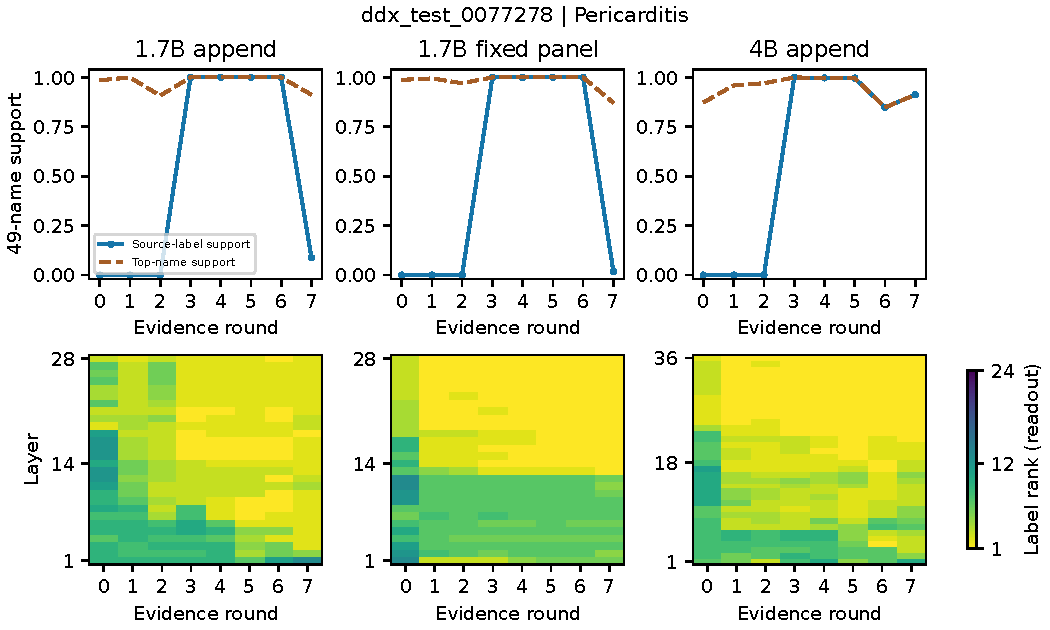
\includegraphics[width=.96\linewidth]{figures/ddx_test_0077278.pdf}\end{center}

{\small\begin{longtable}{>{\raggedright\arraybackslash}p{.07\textwidth}>{\raggedright\arraybackslash}p{.415\textwidth}>{\raggedright\arraybackslash}p{.415\textwidth}}\toprule Round & Newly revealed source evidence & Native top / label support / final-layer probe top \\ \midrule\endhead

0 & Are you experiencing shortness of breath or difficulty breathing in a significant way? Yes & 1.7B append: Acute COPD exacerbation / infection / 0.0000 / Bronchitis\newline 1.7B panel: Acute pulmonary edema / 0.0000 / Guillain-Barr\'{e} syndrome\newline 4B append: Bronchitis / 0.0000 / Bronchitis \\ 

1 & Do you have pain somewhere, related to your reason for consulting? Yes; Characterize your pain: a knife stroke; sharp; Do you feel pain somewhere? lower chest; breast(R); How intense is the pain? Recorded scale value 8 on the dataset's 0-10 scale; endpoint meanings are unspecified; Does the pain radiate to another location? nowhere; How precisely is the pain located? Recorded scale value 7 on the dataset's 0-10 scale; endpoint meanings are unspecified; How fast did the pain appear? Recorded scale value 7 on the dataset's 0-10 scale; endpoint meanings are unspecified & 1.7B append: Boerhaave / 0.0000 / Pulmonary embolism\newline 1.7B panel: Acute COPD exacerbation / infection / 0.0000 / Pericarditis\newline 4B append: Bronchospasm / acute asthma exacerbation / 0.0000 / Pericarditis \\ 

2 & Do you have pain that is increased when you breathe in deeply? Yes & 1.7B append: Bronchospasm / acute asthma exacerbation / 0.0000 / Acute dystonic reactions\newline 1.7B panel: Acute COPD exacerbation / infection / 0.0000 / Pericarditis\newline 4B append: Bronchospasm / acute asthma exacerbation / 0.0000 / Pericarditis \\ 

3 & Have you ever had a pericarditis? Yes & 1.7B append: Pericarditis / 1.0000 / SLE\newline 1.7B panel: Pericarditis / 1.0000 / Pericarditis\newline 4B append: Pericarditis / 0.9998 / Pericarditis \\ 

4 & Have you traveled out of the country in the last 4 weeks? No & 1.7B append: Pericarditis / 1.0000 / SLE\newline 1.7B panel: Pericarditis / 1.0000 / Pericarditis\newline 4B append: Pericarditis / 0.9974 / Pericarditis \\ 

5 & Do you feel your heart is beating fast (racing), irregularly (missing a beat) or do you feel palpitations? Yes & 1.7B append: Pericarditis / 0.9999 / SLE\newline 1.7B panel: Pericarditis / 1.0000 / Pericarditis\newline 4B append: Pericarditis / 0.9966 / Pericarditis \\ 

6 & Are your symptoms worse when lying down and alleviated while sitting up? Yes & 1.7B append: Pericarditis / 1.0000 / Pericarditis\newline 1.7B panel: Pericarditis / 1.0000 / Pericarditis\newline 4B append: Pericarditis / 0.8480 / Pericarditis \\ 

7 & Have you recently had a viral infection? Yes & 1.7B append: Boerhaave / 0.0876 / Pulmonary embolism\newline 1.7B panel: Acute COPD exacerbation / infection / 0.0179 / Pericarditis\newline 4B append: Pericarditis / 0.9124 / Pericarditis \\ 

\bottomrule\end{longtable}}

\clearpage\subsection{ddx\_test\_0079685 -- Guillain-Barr\'{e} syndrome}
\label{case:ddx_test_0079685}

Source label: Guillain-Barr\'{e} syndrome. Family: neurologic. Evidence updates: 7. All facts below are source-recorded; their order is acquisition order.

\begin{center}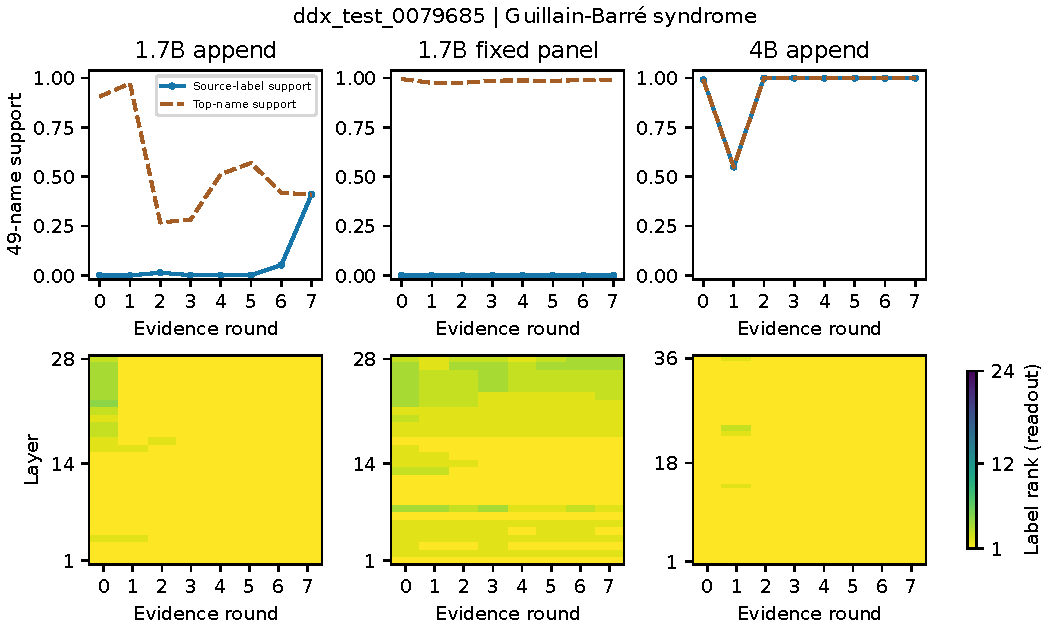
\includegraphics[width=.96\linewidth]{figures/ddx_test_0079685.pdf}\end{center}

{\small\begin{longtable}{>{\raggedright\arraybackslash}p{.07\textwidth}>{\raggedright\arraybackslash}p{.415\textwidth}>{\raggedright\arraybackslash}p{.415\textwidth}}\toprule Round & Newly revealed source evidence & Native top / label support / final-layer probe top \\ \midrule\endhead

0 & Have you had weakness or paralysis on one side of the face, which may still be present or completely resolved? Yes & 1.7B append: Acute COPD exacerbation / infection / 0.0000 / Bronchitis\newline 1.7B panel: Acute COPD exacerbation / infection / 0.0000 / Myasthenia gravis\newline 4B append: Guillain-Barr\'{e} syndrome / 0.9914 / Guillain-Barr\'{e} syndrome \\ 

1 & Do you have numbness, loss of sensation or tingling in the feet? Yes & 1.7B append: Acute rhinosinusitis / 0.0000 / Guillain-Barr\'{e} syndrome\newline 1.7B panel: Acute COPD exacerbation / infection / 0.0000 / Myasthenia gravis\newline 4B append: Guillain-Barr\'{e} syndrome / 0.5498 / Myasthenia gravis \\ 

2 & Did you previously, or do you currently, have any weakness/paralysis in one or more of your limbs or in your face? Yes & 1.7B append: Acute rhinosinusitis / 0.0139 / Guillain-Barr\'{e} syndrome\newline 1.7B panel: Acute COPD exacerbation / infection / 0.0000 / Myasthenia gravis\newline 4B append: Guillain-Barr\'{e} syndrome / 1.0000 / Guillain-Barr\'{e} syndrome \\ 

3 & Do you feel weakness in both arms and/or both legs? Yes & 1.7B append: Myasthenia gravis / 0.0015 / Guillain-Barr\'{e} syndrome\newline 1.7B panel: Acute COPD exacerbation / infection / 0.0000 / Myasthenia gravis\newline 4B append: Guillain-Barr\'{e} syndrome / 1.0000 / Guillain-Barr\'{e} syndrome \\ 

4 & Have you recently had a viral infection? Yes & 1.7B append: Acute rhinosinusitis / 0.0000 / Guillain-Barr\'{e} syndrome\newline 1.7B panel: Acute COPD exacerbation / infection / 0.0000 / Myasthenia gravis\newline 4B append: Guillain-Barr\'{e} syndrome / 1.0000 / Guillain-Barr\'{e} syndrome \\ 

5 & Have you recently had numbness, loss of sensation or tingling, in both arms and legs and around your mouth? Yes & 1.7B append: Acute rhinosinusitis / 0.0008 / Guillain-Barr\'{e} syndrome\newline 1.7B panel: Acute COPD exacerbation / infection / 0.0000 / Myasthenia gravis\newline 4B append: Guillain-Barr\'{e} syndrome / 1.0000 / Guillain-Barr\'{e} syndrome \\ 

6 & Have you traveled out of the country in the last 4 weeks? No & 1.7B append: Acute COPD exacerbation / infection / 0.0526 / Guillain-Barr\'{e} syndrome\newline 1.7B panel: Acute COPD exacerbation / infection / 0.0000 / Myasthenia gravis\newline 4B append: Guillain-Barr\'{e} syndrome / 1.0000 / Guillain-Barr\'{e} syndrome \\ 

7 & Do you currently, or did you ever, have numbness, loss of sensitivity or tingling anywhere on your body? Yes & 1.7B append: Guillain-Barr\'{e} syndrome / 0.4097 / Guillain-Barr\'{e} syndrome\newline 1.7B panel: Acute COPD exacerbation / infection / 0.0000 / Myasthenia gravis\newline 4B append: Guillain-Barr\'{e} syndrome / 1.0000 / Guillain-Barr\'{e} syndrome \\ 

\bottomrule\end{longtable}}

\clearpage\subsection{ddx\_test\_0084538 -- Inguinal hernia}
\label{case:ddx_test_0084538}

Source label: Inguinal hernia. Family: digestive. Evidence updates: 8. All facts below are source-recorded; their order is acquisition order.

\begin{center}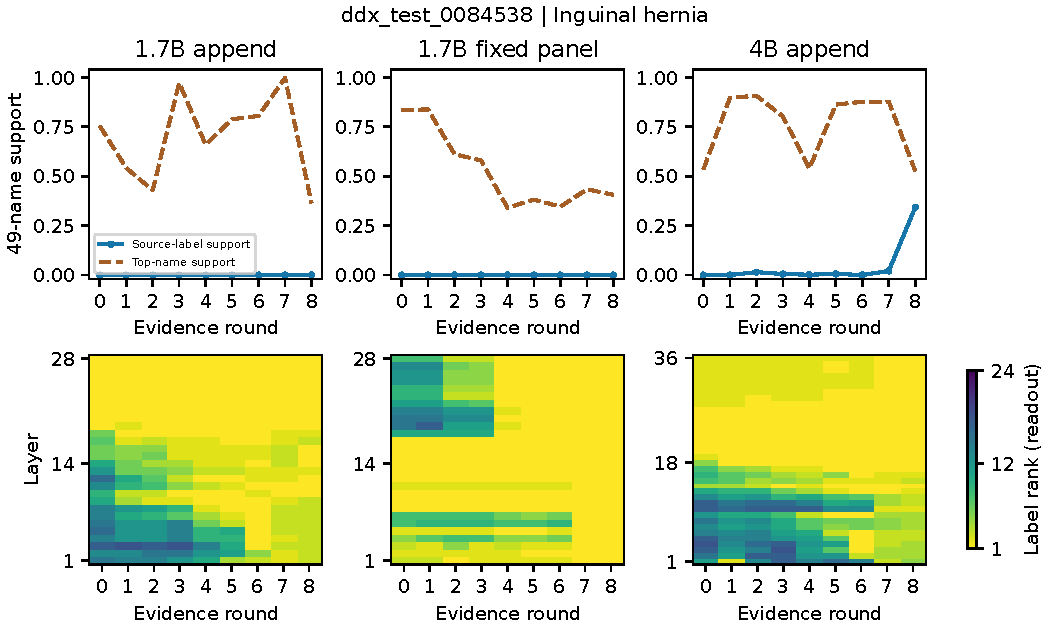
\includegraphics[width=.96\linewidth]{figures/ddx_test_0084538.pdf}\end{center}

{\small\begin{longtable}{>{\raggedright\arraybackslash}p{.07\textwidth}>{\raggedright\arraybackslash}p{.415\textwidth}>{\raggedright\arraybackslash}p{.415\textwidth}}\toprule Round & Newly revealed source evidence & Native top / label support / final-layer probe top \\ \midrule\endhead

0 & Do you have any lesions, redness or problems on your skin that you believe are related to the condition you are consulting for? Yes; What color is the rash? pale; Do your lesions peel off? No; Is the rash swollen? Recorded scale value 4 on the dataset's 0-10 scale; endpoint meanings are unspecified; Where is the affected region located? iliac fossa(R); iliac fossa(L); How intense is the pain caused by the rash? Recorded scale value 6 on the dataset's 0-10 scale; endpoint meanings are unspecified; Is the lesion (or are the lesions) larger than 1cm? Yes; How severe is the itching? Recorded scale value 0 on the dataset's 0-10 scale; endpoint meanings are unspecified & 1.7B append: Localized edema / 0.0001 / Inguinal hernia\newline 1.7B panel: Acute COPD exacerbation / infection / 0.0000 / Myasthenia gravis\newline 4B append: Pulmonary embolism / 0.0000 / SLE \\ 

1 & Were you born prematurely or did you suffer any complication at birth? Yes & 1.7B append: Acute rhinosinusitis / 0.0000 / Inguinal hernia\newline 1.7B panel: Acute COPD exacerbation / infection / 0.0000 / Myasthenia gravis\newline 4B append: Pulmonary embolism / 0.0003 / SLE \\ 

2 & Do you feel your abdomen is bloated or distended (swollen due to pressure from inside)? Yes & 1.7B append: Acute pulmonary edema / 0.0001 / Inguinal hernia\newline 1.7B panel: Acute COPD exacerbation / infection / 0.0000 / HIV (initial infection)\newline 4B append: Pulmonary embolism / 0.0148 / SLE \\ 

3 & Have you been able to pass stools or gas since your symptoms increased? Yes & 1.7B append: Localized edema / 0.0000 / Inguinal hernia\newline 1.7B panel: Acute COPD exacerbation / infection / 0.0000 / HIV (initial infection)\newline 4B append: Pulmonary embolism / 0.0053 / SLE \\ 

4 & Do you have intense coughing fits? Yes & 1.7B append: Pneumonia / 0.0000 / Inguinal hernia\newline 1.7B panel: Acute pulmonary edema / 0.0000 / Inguinal hernia\newline 4B append: Pulmonary embolism / 0.0018 / SLE \\ 

5 & Are the symptoms or pain increased with coughing, with an effort like lifting a weight or from forcing a bowel movement? Yes & 1.7B append: Pneumonia / 0.0000 / Inguinal hernia\newline 1.7B panel: Acute pulmonary edema / 0.0000 / Inguinal hernia\newline 4B append: Pneumonia / 0.0059 / SLE \\ 

6 & Have you traveled out of the country in the last 4 weeks? No & 1.7B append: Pneumonia / 0.0000 / Inguinal hernia\newline 1.7B panel: Acute pulmonary edema / 0.0000 / Inguinal hernia\newline 4B append: Pneumonia / 0.0003 / SLE \\ 

7 & Do you have pain somewhere, related to your reason for consulting? Yes; Characterize your pain: heavy; Do you feel pain somewhere? iliac fossa(R); iliac fossa(L); hip(R); hip(L); How intense is the pain? Recorded scale value 3 on the dataset's 0-10 scale; endpoint meanings are unspecified; Does the pain radiate to another location? nowhere; How precisely is the pain located? Recorded scale value 0 on the dataset's 0-10 scale; endpoint meanings are unspecified; How fast did the pain appear? Recorded scale value 1 on the dataset's 0-10 scale; endpoint meanings are unspecified & 1.7B append: Localized edema / 0.0000 / Inguinal hernia\newline 1.7B panel: Acute pulmonary edema / 0.0000 / Inguinal hernia\newline 4B append: Pneumonia / 0.0207 / Inguinal hernia \\ 

8 & Are you significantly overweight compared to people of the same height as you? Yes & 1.7B append: Localized edema / 0.0000 / Inguinal hernia\newline 1.7B panel: Acute pulmonary edema / 0.0000 / Inguinal hernia\newline 4B append: Pneumonia / 0.3426 / Inguinal hernia \\ 

\bottomrule\end{longtable}}

\clearpage\subsection{ddx\_test\_0101113 -- Spontaneous pneumothorax}
\label{case:ddx_test_0101113}

Source label: Spontaneous pneumothorax. Family: respiratory. Evidence updates: 5. All facts below are source-recorded; their order is acquisition order.

\begin{center}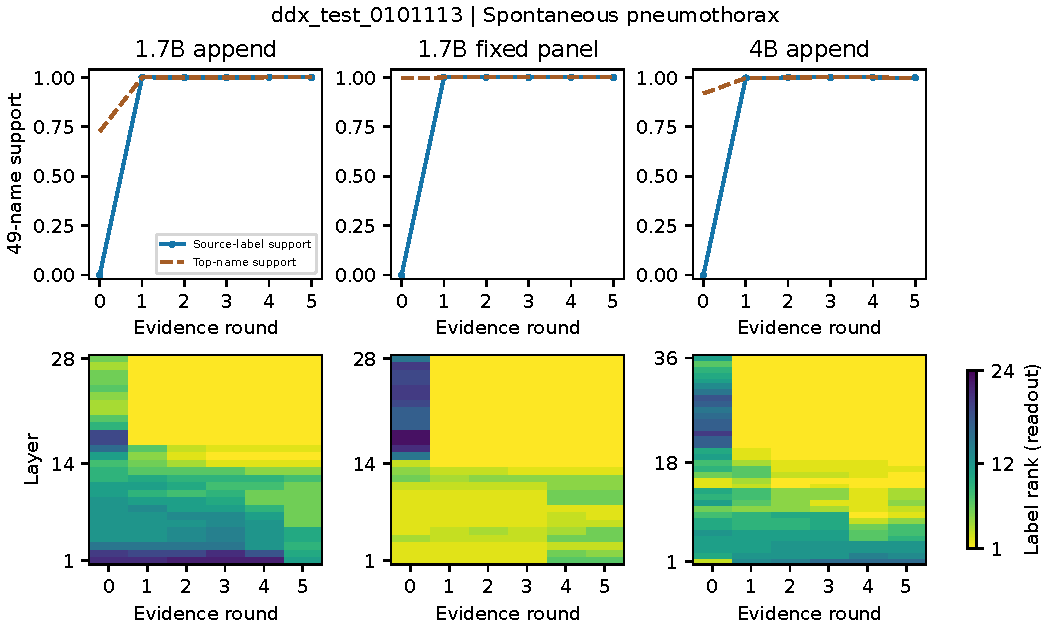
\includegraphics[width=.96\linewidth]{figures/ddx_test_0101113.pdf}\end{center}

{\small\begin{longtable}{>{\raggedright\arraybackslash}p{.07\textwidth}>{\raggedright\arraybackslash}p{.415\textwidth}>{\raggedright\arraybackslash}p{.415\textwidth}}\toprule Round & Newly revealed source evidence & Native top / label support / final-layer probe top \\ \midrule\endhead

0 & Do you have pain somewhere, related to your reason for consulting? Yes; Characterize your pain: heartbreaking; a knife stroke; Do you feel pain somewhere? lower chest; side of the chest(R); upper chest; breast(R); breast(L); How intense is the pain? Recorded scale value 7 on the dataset's 0-10 scale; endpoint meanings are unspecified; Does the pain radiate to another location? nowhere; How precisely is the pain located? Recorded scale value 6 on the dataset's 0-10 scale; endpoint meanings are unspecified; How fast did the pain appear? Recorded scale value 6 on the dataset's 0-10 scale; endpoint meanings are unspecified & 1.7B append: Acute pulmonary edema / 0.0001 / Pericarditis\newline 1.7B panel: Acute COPD exacerbation / infection / 0.0000 / Boerhaave\newline 4B append: Pericarditis / 0.0000 / Pericarditis \\ 

1 & Have you ever had a spontaneous pneumothorax? Yes & 1.7B append: Spontaneous pneumothorax / 1.0000 / Spontaneous pneumothorax\newline 1.7B panel: Spontaneous pneumothorax / 1.0000 / Spontaneous pneumothorax\newline 4B append: Spontaneous pneumothorax / 0.9969 / Spontaneous pneumothorax \\ 

2 & Do you have pain that is increased when you breathe in deeply? Yes & 1.7B append: Spontaneous pneumothorax / 0.9994 / Spontaneous pneumothorax\newline 1.7B panel: Spontaneous pneumothorax / 1.0000 / Spontaneous pneumothorax\newline 4B append: Spontaneous pneumothorax / 0.9997 / Spontaneous pneumothorax \\ 

3 & Do you smoke cigarettes? Yes & 1.7B append: Spontaneous pneumothorax / 0.9994 / Spontaneous pneumothorax\newline 1.7B panel: Spontaneous pneumothorax / 1.0000 / Spontaneous pneumothorax\newline 4B append: Spontaneous pneumothorax / 1.0000 / Spontaneous pneumothorax \\ 

4 & Have you traveled out of the country in the last 4 weeks? North America & 1.7B append: Spontaneous pneumothorax / 0.9999 / Spontaneous pneumothorax\newline 1.7B panel: Spontaneous pneumothorax / 1.0000 / Spontaneous pneumothorax\newline 4B append: Spontaneous pneumothorax / 1.0000 / Spontaneous pneumothorax \\ 

5 & Do you have symptoms that are increased with physical exertion but alleviated with rest? Yes & 1.7B append: Spontaneous pneumothorax / 1.0000 / Spontaneous pneumothorax\newline 1.7B panel: Spontaneous pneumothorax / 1.0000 / Spontaneous pneumothorax\newline 4B append: Spontaneous pneumothorax / 0.9979 / Spontaneous pneumothorax \\ 

\bottomrule\end{longtable}}

\clearpage\subsection{ddx\_test\_0108184 -- Guillain-Barr\'{e} syndrome}
\label{case:ddx_test_0108184}

Source label: Guillain-Barr\'{e} syndrome. Family: neurologic. Evidence updates: 6. All facts below are source-recorded; their order is acquisition order.

\begin{center}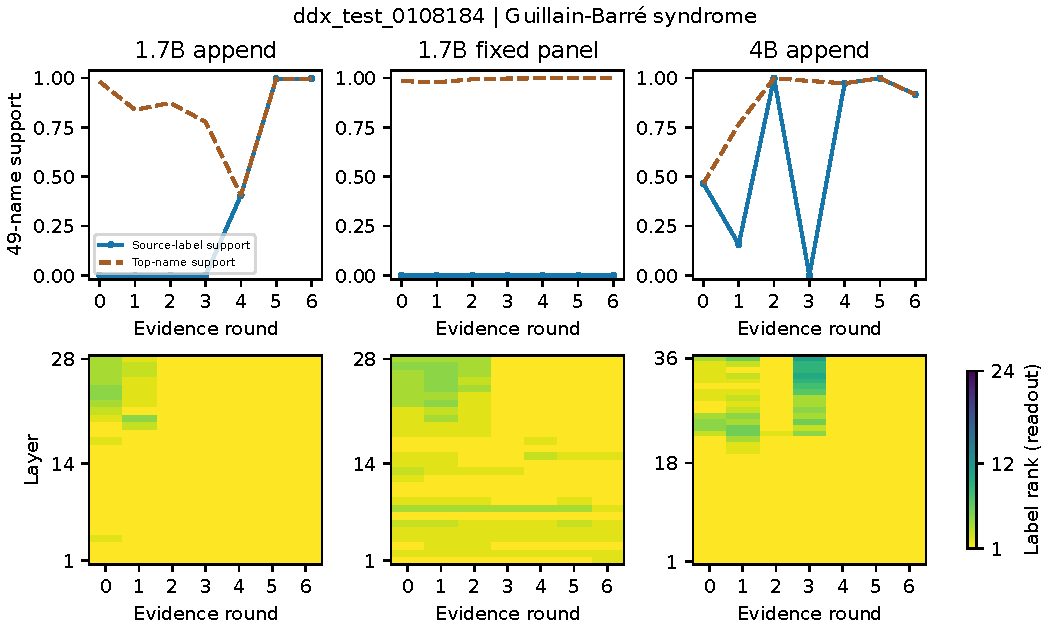
\includegraphics[width=.96\linewidth]{figures/ddx_test_0108184.pdf}\end{center}

{\small\begin{longtable}{>{\raggedright\arraybackslash}p{.07\textwidth}>{\raggedright\arraybackslash}p{.415\textwidth}>{\raggedright\arraybackslash}p{.415\textwidth}}\toprule Round & Newly revealed source evidence & Native top / label support / final-layer probe top \\ \midrule\endhead

0 & Do you currently, or did you ever, have numbness, loss of sensitivity or tingling anywhere on your body? Yes & 1.7B append: Acute COPD exacerbation / infection / 0.0000 / Acute dystonic reactions\newline 1.7B panel: Acute COPD exacerbation / infection / 0.0000 / Myasthenia gravis\newline 4B append: Guillain-Barr\'{e} syndrome / 0.4657 / Possible NSTEMI / STEMI \\ 

1 & Have you traveled out of the country in the last 4 weeks? No & 1.7B append: Acute rhinosinusitis / 0.0000 / Acute dystonic reactions\newline 1.7B panel: Acute COPD exacerbation / infection / 0.0000 / Myasthenia gravis\newline 4B append: Acute rhinosinusitis / 0.1571 / Possible NSTEMI / STEMI \\ 

2 & Do you feel weakness in both arms and/or both legs? Yes & 1.7B append: Bronchiolitis / 0.0000 / Guillain-Barr\'{e} syndrome\newline 1.7B panel: Acute COPD exacerbation / infection / 0.0000 / Myasthenia gravis\newline 4B append: Guillain-Barr\'{e} syndrome / 1.0000 / Guillain-Barr\'{e} syndrome \\ 

3 & Are you experiencing shortness of breath or difficulty breathing in a significant way? Yes & 1.7B append: Acute pulmonary edema / 0.0000 / Guillain-Barr\'{e} syndrome\newline 1.7B panel: Acute pulmonary edema / 0.0000 / Guillain-Barr\'{e} syndrome\newline 4B append: Pulmonary embolism / 0.0000 / Acute pulmonary edema \\ 

4 & Have you recently had numbness, loss of sensation or tingling, in both arms and legs and around your mouth? Yes & 1.7B append: Guillain-Barr\'{e} syndrome / 0.4066 / Guillain-Barr\'{e} syndrome\newline 1.7B panel: Acute pulmonary edema / 0.0000 / Guillain-Barr\'{e} syndrome\newline 4B append: Guillain-Barr\'{e} syndrome / 0.9741 / Guillain-Barr\'{e} syndrome \\ 

5 & Did you previously, or do you currently, have any weakness/paralysis in one or more of your limbs or in your face? Yes & 1.7B append: Guillain-Barr\'{e} syndrome / 0.9965 / Guillain-Barr\'{e} syndrome\newline 1.7B panel: Acute pulmonary edema / 0.0000 / Guillain-Barr\'{e} syndrome\newline 4B append: Guillain-Barr\'{e} syndrome / 0.9998 / Guillain-Barr\'{e} syndrome \\ 

6 & Have you recently had a viral infection? Yes & 1.7B append: Guillain-Barr\'{e} syndrome / 0.9973 / Guillain-Barr\'{e} syndrome\newline 1.7B panel: Acute pulmonary edema / 0.0000 / Guillain-Barr\'{e} syndrome\newline 4B append: Guillain-Barr\'{e} syndrome / 0.9173 / Guillain-Barr\'{e} syndrome \\ 

\bottomrule\end{longtable}}

\clearpage\subsection{ddx\_test\_0110714 -- Pulmonary embolism}
\label{case:ddx_test_0110714}

Source label: Pulmonary embolism. Family: respiratory. Evidence updates: 8. All facts below are source-recorded; their order is acquisition order.

\begin{center}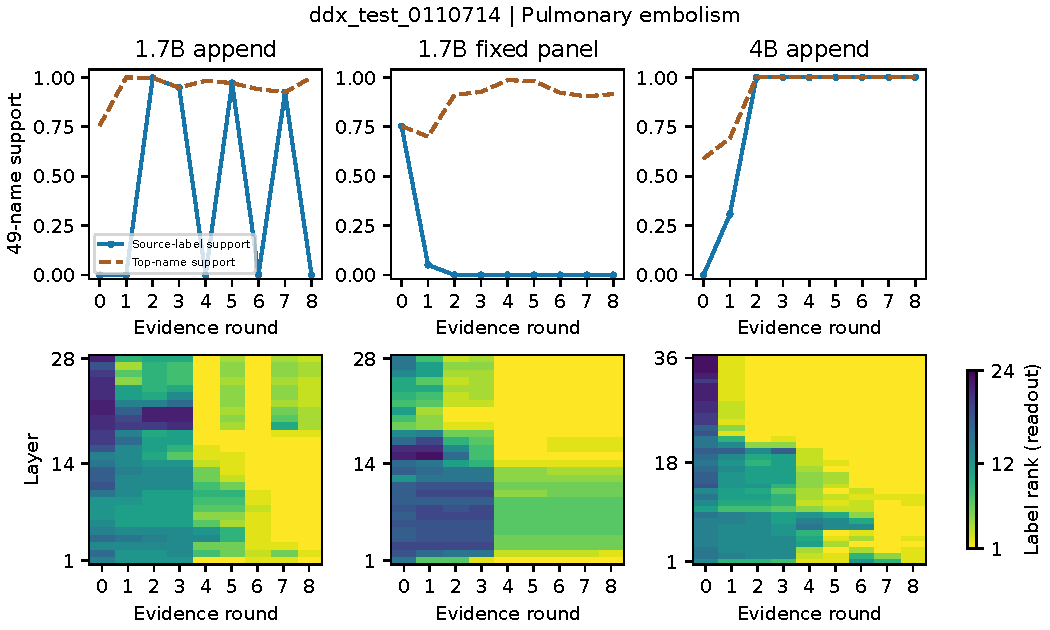
\includegraphics[width=.96\linewidth]{figures/ddx_test_0110714.pdf}\end{center}

{\small\begin{longtable}{>{\raggedright\arraybackslash}p{.07\textwidth}>{\raggedright\arraybackslash}p{.415\textwidth}>{\raggedright\arraybackslash}p{.415\textwidth}}\toprule Round & Newly revealed source evidence & Native top / label support / final-layer probe top \\ \midrule\endhead

0 & Do you have pain that is increased when you breathe in deeply? Yes & 1.7B append: Acute COPD exacerbation / infection / 0.0000 / Bronchitis\newline 1.7B panel: Pulmonary embolism / 0.7534 / SLE\newline 4B append: Acute pulmonary edema / 0.0000 / Bronchitis \\ 

1 & Do you have swelling in one or more areas of your body? Yes; Where is the swelling located? posterior aspect of the ankle(R); posterior aspect of the ankle(L); calf(L) & 1.7B append: Localized edema / 0.0000 / Acute pulmonary edema\newline 1.7B panel: Acute COPD exacerbation / infection / 0.0512 / Myasthenia gravis\newline 4B append: Localized edema / 0.3071 / Acute pulmonary edema \\ 

2 & Have you ever had deep vein thrombosis (DVT)? Yes & 1.7B append: Pulmonary embolism / 0.9975 / Anemia\newline 1.7B panel: Acute COPD exacerbation / infection / 0.0001 / Myasthenia gravis\newline 4B append: Pulmonary embolism / 1.0000 / Pulmonary embolism \\ 

3 & Have you traveled out of the country in the last 4 weeks? North America & 1.7B append: Pulmonary embolism / 0.9483 / Acute pulmonary edema\newline 1.7B panel: Acute COPD exacerbation / infection / 0.0000 / Myasthenia gravis\newline 4B append: Pulmonary embolism / 1.0000 / Pulmonary embolism \\ 

4 & Do you have pain somewhere, related to your reason for consulting? Yes; Characterize your pain: a knife stroke; sharp; Do you feel pain somewhere? side of the chest(R); side of the chest(L); scapula(L); posterior chest wall(R); posterior chest wall(L); How intense is the pain? Recorded scale value 10 on the dataset's 0-10 scale; endpoint meanings are unspecified; Does the pain radiate to another location? side of the chest(R); side of the chest(L); scapula(R); breast(R); posterior chest wall(R); How precisely is the pain located? Recorded scale value 4 on the dataset's 0-10 scale; endpoint meanings are unspecified; How fast did the pain appear? Recorded scale value 10 on the dataset's 0-10 scale; endpoint meanings are unspecified & 1.7B append: Boerhaave / 0.0000 / Pulmonary embolism\newline 1.7B panel: Acute COPD exacerbation / infection / 0.0000 / Pulmonary embolism\newline 4B append: Pulmonary embolism / 1.0000 / Pulmonary embolism \\ 

5 & Did you lose consciousness? Yes & 1.7B append: Pulmonary embolism / 0.9713 / Acute pulmonary edema\newline 1.7B panel: Acute COPD exacerbation / infection / 0.0000 / Pulmonary embolism\newline 4B append: Pulmonary embolism / 1.0000 / Pulmonary embolism \\ 

6 & Have you been coughing up blood? Yes & 1.7B append: Boerhaave / 0.0026 / Pulmonary embolism\newline 1.7B panel: Acute COPD exacerbation / infection / 0.0000 / Pulmonary embolism\newline 4B append: Pulmonary embolism / 1.0000 / Pulmonary embolism \\ 

7 & Have you been unable to move or get up for more than 3 consecutive days within the last 4 weeks? Yes & 1.7B append: Pulmonary embolism / 0.9253 / Acute pulmonary edema\newline 1.7B panel: Acute COPD exacerbation / infection / 0.0000 / Pulmonary embolism\newline 4B append: Pulmonary embolism / 1.0000 / Pulmonary embolism \\ 

8 & Have you had surgery within the last month? Yes & 1.7B append: Localized edema / 0.0001 / Acute pulmonary edema\newline 1.7B panel: Acute COPD exacerbation / infection / 0.0000 / Pulmonary embolism\newline 4B append: Pulmonary embolism / 1.0000 / Pulmonary embolism \\ 

\bottomrule\end{longtable}}

\clearpage\subsection{ddx\_test\_0123136 -- GERD}
\label{case:ddx_test_0123136}

Source label: GERD. Family: digestive. Evidence updates: 8. All facts below are source-recorded; their order is acquisition order.

\begin{center}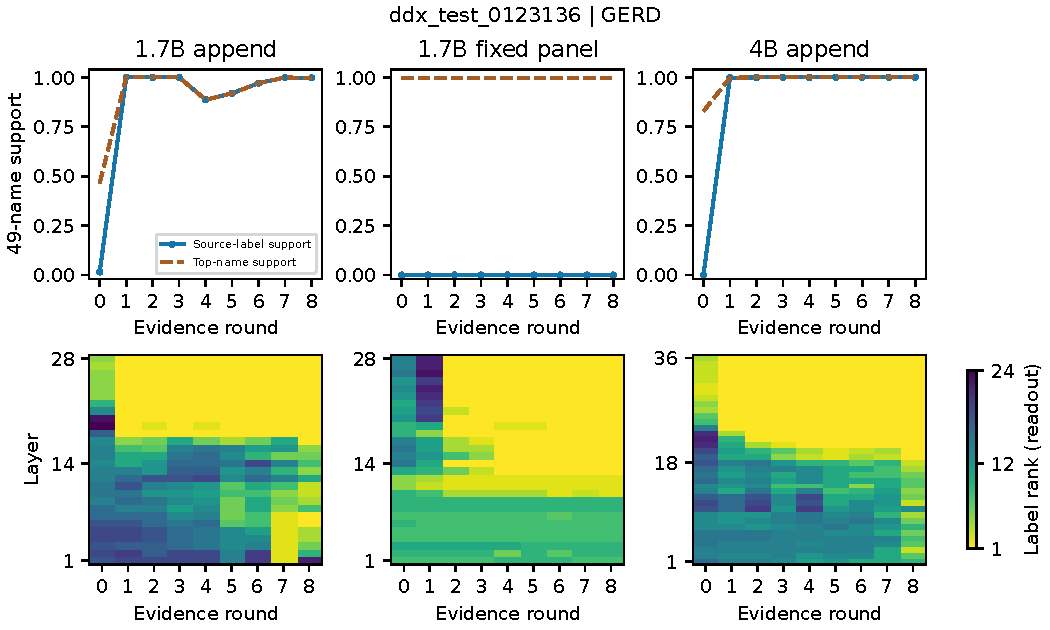
\includegraphics[width=.96\linewidth]{figures/ddx_test_0123136.pdf}\end{center}

{\small\begin{longtable}{>{\raggedright\arraybackslash}p{.07\textwidth}>{\raggedright\arraybackslash}p{.415\textwidth}>{\raggedright\arraybackslash}p{.415\textwidth}}\toprule Round & Newly revealed source evidence & Native top / label support / final-layer probe top \\ \midrule\endhead

0 & Do you have pain somewhere, related to your reason for consulting? Yes; Characterize your pain: sensitive; burning; sickening; scary; Do you feel pain somewhere? upper chest; hypochondrium(L); epigastric; How intense is the pain? Recorded scale value 4 on the dataset's 0-10 scale; endpoint meanings are unspecified; Does the pain radiate to another location? upper chest; How precisely is the pain located? Recorded scale value 2 on the dataset's 0-10 scale; endpoint meanings are unspecified; How fast did the pain appear? Recorded scale value 2 on the dataset's 0-10 scale; endpoint meanings are unspecified & 1.7B append: Acute pulmonary edema / 0.0161 / Stable angina\newline 1.7B panel: Acute COPD exacerbation / infection / 0.0000 / Pericarditis\newline 4B append: Acute pulmonary edema / 0.0000 / Pericarditis \\ 

1 & Do you have a hiatal hernia? Yes & 1.7B append: GERD / 1.0000 / GERD\newline 1.7B panel: Acute COPD exacerbation / infection / 0.0000 / Pericarditis\newline 4B append: GERD / 0.9988 / GERD \\ 

2 & Do you have symptoms that get worse after eating? Yes & 1.7B append: GERD / 1.0000 / GERD\newline 1.7B panel: Acute COPD exacerbation / infection / 0.0000 / GERD\newline 4B append: GERD / 1.0000 / GERD \\ 

3 & Do you think you are pregnant or are you currently pregnant? Yes & 1.7B append: GERD / 1.0000 / GERD\newline 1.7B panel: Acute COPD exacerbation / infection / 0.0000 / GERD\newline 4B append: GERD / 1.0000 / GERD \\ 

4 & Have you recently thrown up blood or something resembling coffee beans? Yes & 1.7B append: GERD / 0.8872 / GERD\newline 1.7B panel: Acute COPD exacerbation / infection / 0.0000 / GERD\newline 4B append: GERD / 1.0000 / GERD \\ 

5 & Do you smoke cigarettes? Yes & 1.7B append: GERD / 0.9196 / GERD\newline 1.7B panel: Acute COPD exacerbation / infection / 0.0000 / GERD\newline 4B append: GERD / 1.0000 / GERD \\ 

6 & Do you have asthma or have you ever had to use a bronchodilator in the past? Yes & 1.7B append: GERD / 0.9707 / GERD\newline 1.7B panel: Acute COPD exacerbation / infection / 0.0000 / GERD\newline 4B append: GERD / 1.0000 / GERD \\ 

7 & Have you traveled out of the country in the last 4 weeks? No & 1.7B append: GERD / 0.9998 / GERD\newline 1.7B panel: Acute COPD exacerbation / infection / 0.0000 / GERD\newline 4B append: GERD / 1.0000 / GERD \\ 

8 & Do you have a burning sensation that starts in your stomach then goes up into your throat, and can be associated with a bitter taste in your mouth? Yes & 1.7B append: GERD / 0.9977 / GERD\newline 1.7B panel: Acute COPD exacerbation / infection / 0.0000 / GERD\newline 4B append: GERD / 1.0000 / GERD \\ 

\bottomrule\end{longtable}}

\clearpage\subsection{ddx\_test\_0134351 -- Viral pharyngitis}
\label{case:ddx_test_0134351}

Source label: Viral pharyngitis. Family: ent. Evidence updates: 5. All facts below are source-recorded; their order is acquisition order.

\begin{center}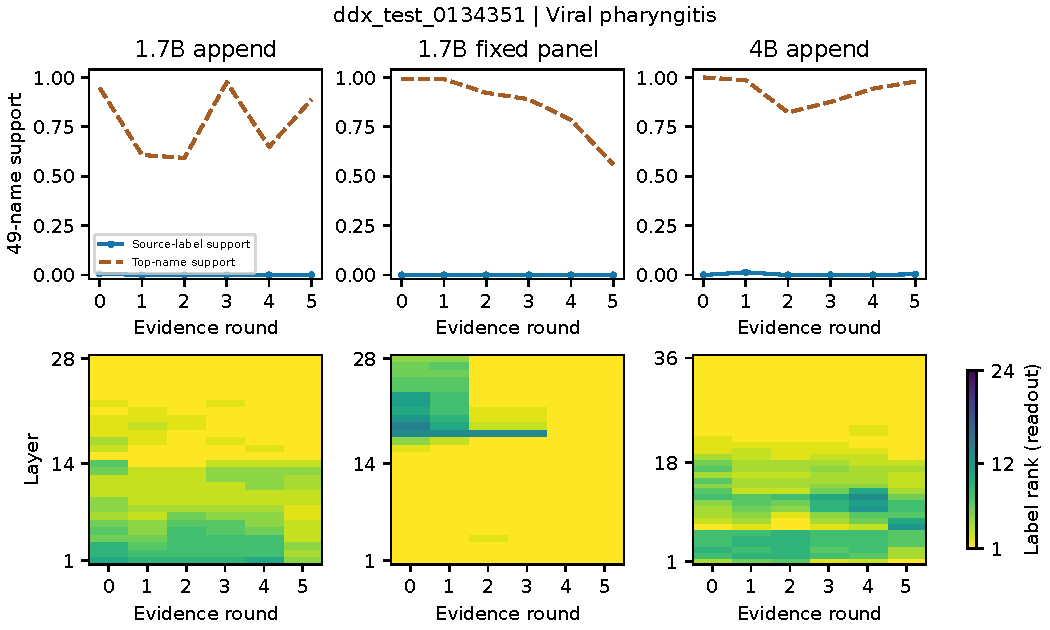
\includegraphics[width=.96\linewidth]{figures/ddx_test_0134351.pdf}\end{center}

{\small\begin{longtable}{>{\raggedright\arraybackslash}p{.07\textwidth}>{\raggedright\arraybackslash}p{.415\textwidth}>{\raggedright\arraybackslash}p{.415\textwidth}}\toprule Round & Newly revealed source evidence & Native top / label support / final-layer probe top \\ \midrule\endhead

0 & Do you have pain somewhere, related to your reason for consulting? Yes; Characterize your pain: sensitive; burning; Do you feel pain somewhere? tonsil(R); tonsil(L); palace; pharynx; under the jaw; How intense is the pain? Recorded scale value 9 on the dataset's 0-10 scale; endpoint meanings are unspecified; Does the pain radiate to another location? nowhere; How precisely is the pain located? Recorded scale value 7 on the dataset's 0-10 scale; endpoint meanings are unspecified; How fast did the pain appear? Recorded scale value 3 on the dataset's 0-10 scale; endpoint meanings are unspecified & 1.7B append: Acute rhinosinusitis / 0.0075 / Viral pharyngitis\newline 1.7B panel: Acute COPD exacerbation / infection / 0.0000 / Acute otitis media\newline 4B append: Acute rhinosinusitis / 0.0001 / Viral pharyngitis \\ 

1 & Do you smoke cigarettes? Yes & 1.7B append: Acute laryngitis / 0.0000 / Viral pharyngitis\newline 1.7B panel: Acute COPD exacerbation / infection / 0.0000 / Acute otitis media\newline 4B append: Acute rhinosinusitis / 0.0141 / Viral pharyngitis \\ 

2 & Have you been coughing up blood? Yes & 1.7B append: Acute rhinosinusitis / 0.0001 / Viral pharyngitis\newline 1.7B panel: Acute COPD exacerbation / infection / 0.0000 / Viral pharyngitis\newline 4B append: Acute rhinosinusitis / 0.0000 / Viral pharyngitis \\ 

3 & Have you traveled out of the country in the last 4 weeks? No & 1.7B append: Acute rhinosinusitis / 0.0025 / Viral pharyngitis\newline 1.7B panel: Acute COPD exacerbation / infection / 0.0000 / Viral pharyngitis\newline 4B append: Acute rhinosinusitis / 0.0003 / Viral pharyngitis \\ 

4 & Are you immunosuppressed? Yes & 1.7B append: GERD / 0.0002 / Viral pharyngitis\newline 1.7B panel: Acute COPD exacerbation / infection / 0.0000 / Viral pharyngitis\newline 4B append: Pneumonia / 0.0000 / Viral pharyngitis \\ 

5 & Have you been in contact with a person with similar symptoms in the past 2 weeks? Yes & 1.7B append: Acute rhinosinusitis / 0.0002 / Viral pharyngitis\newline 1.7B panel: Acute COPD exacerbation / infection / 0.0000 / Viral pharyngitis\newline 4B append: Pneumonia / 0.0042 / Viral pharyngitis \\ 

\bottomrule\end{longtable}}

\end{document}
